\section{高次不等式的解法}

不等式$(x-x_1)(x-x_2)\cdots(x-x_n)>0$
(其中$x_1,x_2,\ldots,x_n$是互不相等的实常数)是一元$n$次不等式($n\in\N$). 

若$n=1$,容易写出它的解集为$(x_1,+\infty)$;

若$n=2$,它是一元二次不等式。只要能正确地作出相应的二次函数的图象的草图(关键是开口方向和函数的零点不能弄错),再根据图象写出不等式的解集就没有什么困难了。现在的问题是,能否把这种解法——图象法,推广到$n\ge 3$的情况。

很明显,这时关键在于怎样作出相应函数的图象的草图,让我们先剖析一个实例——作出下列函数图象的草图:
\[y=f(x)=(x+1)(x-1)(x+5)\]

第一步,曲线$y=f(x)$与$x$轴的交点的横坐标(称为\textbf{函数$y=f(x)$的零点})由小到大依次是$-5$,$-1$,1,此时$x$轴被这三个交点分成四段,它们分别对应四个开区间:
\[(-\infty,-5),\quad (-5,-1),\quad (-1,1), \quad (1,+\infty)\]

第二步,研究曲线$y=f(x)$在这四个开区间上分布在横轴的上方还是下方:

在$(1,+\infty)$上,由于$x>1$,所以$x+1>0$, $x-1>0$, $x+5>0\Longrightarrow y>0 \Longrightarrow $曲线$y=f(x)$在$x$轴上方;

在$(-1,1)$上,由于$-1<x<1$,所以$x+1>0$, 
$x-1<0$, $x+5>0\Longrightarrow y<0\Longrightarrow $ 曲线$y=f(x)$在$x$轴下方;

在$(-5,-1)$上,由于$-5<x<-1$,所以$x+1<0$, 
$x-1<0$, $x+5>0\Longrightarrow y>0\Longrightarrow$ 曲线$y=f(x)$在$x$轴上方;

在$(-\infty,-5)$上,由于$x<-5$,所以$x+1<0$, $x-1<0$, $x+5<0\Longrightarrow y<0\Longrightarrow$曲线$y=f(x)$在$x$轴下方;

规律性很明显:曲线$y=f(x)$在上述四个彼此相邻的开区间内,从右到左依次位于$x$轴的上方、下方、上方、下方,而在$x=-5,-1,1$三处曲线与$x$轴相交。

第三步,根据上述分析,作出函数图像的草图(图4.5)。

\begin{figure}[htp]
    \centering
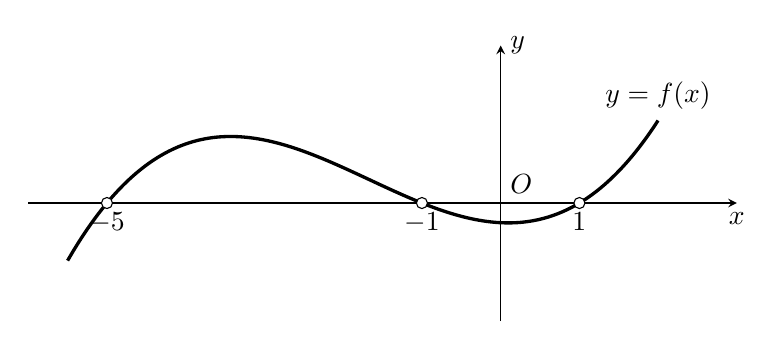
\begin{tikzpicture}[>=stealth]
\draw[->](-6,0)--(3,0)node[below]{$x$};    
\draw[->](0,-1.5)--(0,2)node[right]{$y$};

\draw[domain=-5.5:2, smooth, samples=100, very thick]plot(\x, {0.05*(\x-1)*(\x+1)*(\x+5)})node[above]{$y=f(x)$};

\foreach \x in {1,-1,-5}
{
    \draw[fill=white](\x,0)node[below]{$\x$}circle(2pt);
}
\node [above right]{$O$};
\end{tikzpicture}
    \caption{}
\end{figure}


这种草图上要明确地表示出:
\begin{enumerate}[(a)]
    \item 曲线与$x$轴的交点;
    \item 在某个开区间上函数的那段曲线是在$x$轴的上方还是下方。
\end{enumerate}
除此以外,对草图不必做更细致的要求,例如在某个开区间上函数的最大值(最小值)画得是否确切等都无关紧要。因为在此处我们只关心不等式的解。

通过剖析实例,我们获得了作形如函数
$f(x)=(x-x_1)(x-x_2)\cdots (x-x_n)$
(其中$x_1,x_2,\ldots,x_n$是互不相等的实常数)
图像的草图的一般方法:

第一步,求出曲线$f(x)$与$x$轴交点的横坐标$x_1,x_2,\ldots,x_n$,并把它们由小到大依次标在$x$轴上。标出的$n$个点把$x$轴分成$n+1$个开区间。

第二步,因为曲线$y=f(x)$在这$n+1$个开区间上总是依次上下相间地分布在$x$轴两侧,而且在函数的零点处彼此相连。所以,我们只要确定曲线在最右边的开区间上分布在$x$轴的上侧还是下侧就行了。这是容易办到的,实际上我们总能使$x$的最高次幂的系数为正,曲线总是在$x$轴的上方。

第三步,根据上述分析,作出图象的草图。

\begin{example}
    解不等式:
    \begin{multicols}{2}
\begin{enumerate}[(1)]
    \item $(x-2)(x+1)(x+3)(x+5)>0$
    \item $(x+2)(x-3)(5-x)>0$
\end{enumerate}        
    \end{multicols}
\end{example}

\begin{solution}
\begin{enumerate}[(1)]
    \item 作出函数$y=(x-2)(x+1)(x+3)(x+5)$图象的草图(图4.6)

$\therefore\quad $不等式(1)的解集为$(-\infty,-5)\cup(-3,-1)\cup (2,+\infty)$

\begin{figure}[htp]
    \centering
\begin{minipage}{0.45\textwidth}
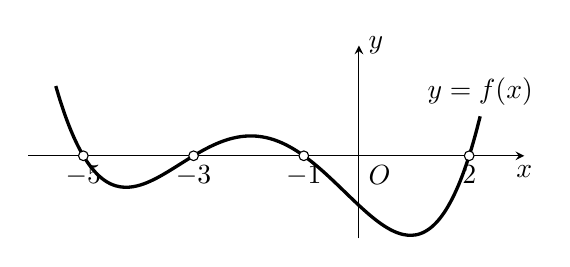
\begin{tikzpicture}[scale=.7, >=stealth]
\draw[->](-6,0)--(3,0)node[below]{$x$};    
\draw[->](0,-1.5)--(0,2)node[right]{$y$};

\draw[domain=-5.5:2.2, smooth, samples=100, very thick]plot(\x, {0.03*(\x-2)*(\x+1)*(\x+5)*(\x+3)})node[above]{$y=f(x)$};

\foreach \x in {-1,-3,-5,2}
{
    \draw[fill=white](\x,0)node[below]{$\x$}circle(2.5pt);
}
\node [below right]{$O$};


 \end{tikzpicture}
    \caption{}   
\end{minipage}\hfill 
\begin{minipage}{0.45\textwidth}
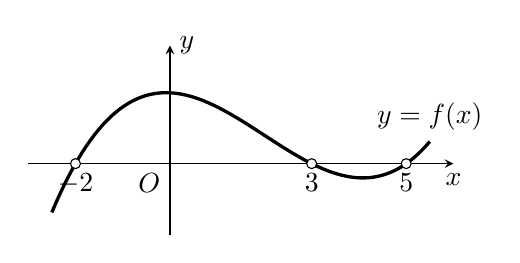
\begin{tikzpicture}[scale=.6, >=stealth]
    \draw[->](-3,0)--(6,0)node[below]{$x$};    
\draw[->](0,-1.5)--(0,2.5)node[right]{$y$};

\draw[domain=-2.5:5.5, smooth, samples=100, very thick]plot(\x, {0.05*(\x-3)*(\x+2)*(\x-5)})node[above]{$y=f(x)$};

\foreach \x in {-2,3,5}
{
    \draw[fill=white](\x,0)node[below]{$\x$}circle(3pt);
}
\node [below left]{$O$};


 \end{tikzpicture}
    \caption{}   
\end{minipage}
\end{figure}


\item 先把原不等式变成与它等价的$(x+2)(x-3)(x-5)<0$,作出函数$y=(x+2)(x-3)(x-5)$图象的草图(图4.7)

$\therefore\quad $解集为$(-\infty,-2)\cup(3,5)$.

\end{enumerate}

注意:在解题中,我们先以$(-1)$乘原不等式,为的是使因式$(5-x)$变成$(x-5)$。这样做可以避免出错。
\end{solution}

\begin{note}
这类不等式的解法可以概括成:找零点,分区间,画草图,写解集。
\end{note}

\begin{example}
解下列不等式:
\begin{enumerate}[(1)]
    \item $(x-4)(x-1)^2(x+2)<0$
    \item $(x+2)(x+1)^2(x-1)^3(x-3)>0$
\end{enumerate}
\end{example}

\begin{analyze}
    此例中函数的解析式$y=(x-4)(x-1)^2(x+2)$出现了重因式,当$x$值由大于1变到小于1的时候(不含$x=1$),$y$的取值符号没有发生变化,如图4.8所示.

\begin{figure}[htp]
    \centering
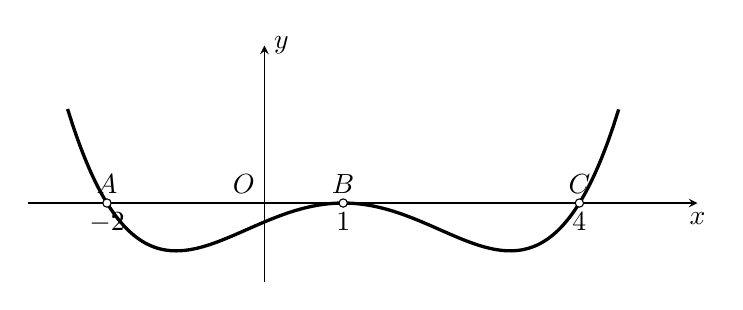
\begin{tikzpicture}[>=stealth]
    \draw[->](-3,0)--(5.5,0)node[below]{$x$};    
\draw[->](0,-1)--(0,2)node[right]{$y$};

\draw[domain=-2.5:4.5, smooth, samples=100, very thick]plot(\x, {0.03*(\x-4)*(\x+2)*(\x-1)*(\x-1)});

\foreach \x/\y in {-2/A,1/B,4/C}
{
    \draw[fill=white](\x,0)node[below]{$\x$}circle(1.5pt)node[above]{$\y$};
}
\node [above left]{$O$};
\end{tikzpicture}
    \caption{}
\end{figure}

    由此,不等式(1)的解集为$(-2,1)\cup (1,4)$.

    基于这个想法,不难得到:若$(x-x_1)$是曲线$y=f(x)$的二重因式,则曲线在点$B(x_1)$处不穿过横轴,若$(x-x_1)$是三重因式,则曲线在点$B(x_1)$处穿过横轴,依次类推。

    对于第(2)题,依上述办法作出函数$y=(x+2)(x+1)(x-1)^3(x-3)$的草图(图4.9).由此可得(2)的解集是$(2-1)\cup (-1,1)\cup (3,+\infty)$.

\begin{figure}[htp]
    \centering
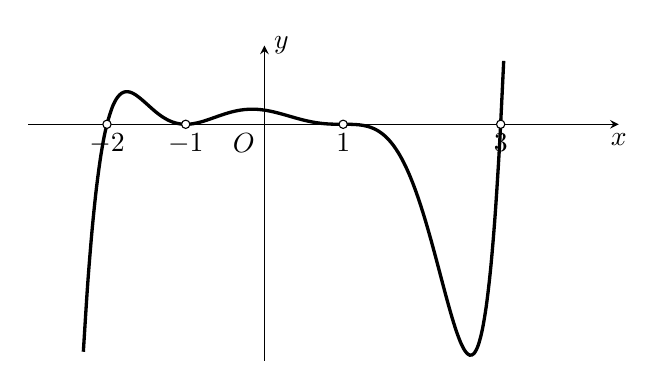
\begin{tikzpicture}[>=stealth]
    \draw[->](-3,0)--(4.5,0)node[below]{$x$};    
\draw[->](0,-3)--(0,1)node[right]{$y$};

\draw[domain=-2.3:3.04, smooth, samples=100, very thick]plot(\x, {0.03*(\x+2)*(\x+1)*(\x+1)*(\x-1)*(\x-1)*(\x-1)*(\x-3)});

\foreach \x in {-2,-1,1,3}
{
    \draw[fill=white](\x,0)node[below]{$\x$}circle(1.5pt);
}
\node [below left]{$O$};

\end{tikzpicture}
    \caption{}
\end{figure}
\end{analyze}

\begin{blk}
    如何解下列不等式:
    \begin{enumerate}[(1)]
        \item $(x+3)(x-2)(x^2-2x-3)<0$;
\item $(x-1)(x^2-x+5)>0$.
    \end{enumerate}
\end{blk}


\begin{example}
    解不等式:$(x+3)(x-2)^2(x+1)^2(x-1)\ge 0$.
\end{example}

\begin{analyze}
    这里出现了“$\ge $”。处理这类问题的办法是:在画函数图象的草图时,只要把曲线与$x$轴的交点画成“实点”即可。
\end{analyze}

\begin{solution}
    作出函数
$y=(x+3)(x-2)^2(x+1)^2(x-1)$的草图(图4.10)。

\begin{figure}[htp]
    \centering
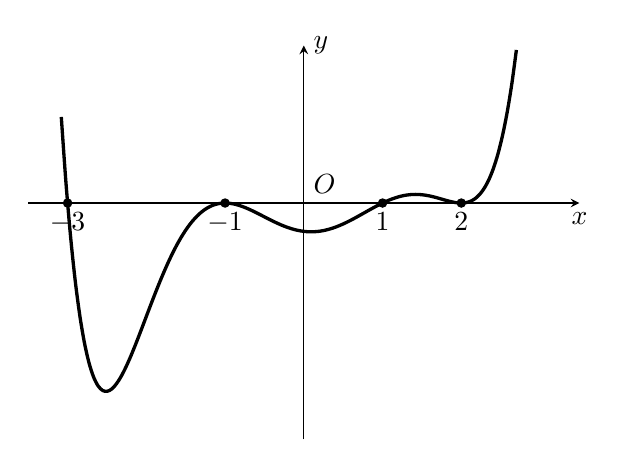
\begin{tikzpicture}[>=stealth]
    \draw[->](-3.5,0)--(3.5,0)node[below]{$x$};    
\draw[->](0,-3)--(0,2)node[right]{$y$};

\draw[domain=-3.08:2.7, smooth, samples=100, very thick]plot(\x, {0.03*(\x-2)*(\x-2)*(\x+1)*(\x+1)*(\x+3)*(\x-1)});

\foreach \x/\y in {-3,-1,1,2}
{
    \draw[fill](\x,0)node[below]{$\x$}circle(1.5pt);
}
\node [above right]{$O$};
\end{tikzpicture}
    \caption{}
\end{figure}

$\therefore\quad $不等式的解集是$(-\infty,-3]\cup\{-1\}\cup [1,+\infty)$
\end{solution}

\section*{习题十}
\begin{center}
    \bfseries A
\end{center}

\begin{enumerate}
    \item 解下列二次不等式:
\begin{multicols}{2}
\begin{enumerate}[(1)]
    \item $x^2+4x-45\ge 0$
    \item $x^2-5ax+6a^2>0$
\end{enumerate}
\end{multicols}

\item \begin{enumerate}[(1)]
    \item 解关于$x$的不等式:$ax^2-2ax+a+3\le 0$
\item 关于$x$的不等式$ax^2+5x+b>0$的解集是$\left(\frac13,\frac12\right)$
,求$a,b$

\item 关于$x$的不等式$ax^2+bx+c>0$ 的解集为$(\alpha,\beta)$, $\alpha >0$, 求关于$x$的不等式$cx^2+bx+a<0$的解集。
\end{enumerate} 

\item 解下列不等式组:
\begin{multicols}{2}
\begin{enumerate}[(1)]
    \item $\begin{cases}
        x^2-3x+2>0\\ x^2-2x-3\le 0
    \end{cases}$
    \item $\begin{cases}
        x-a\ge 0\\ x^2-2x-3<0
    \end{cases}$
\end{enumerate}
\end{multicols}
\item $a$为何值时,不等式组$\begin{cases}
    (x-2)(x-5)\le 0\\ x(x-a)\ge 0
\end{cases}$
的解集为:
\begin{multicols}{2}
\begin{enumerate}[(1)]
    \item $\emptyset$;
    \item 单元素集;
    \item 与第一个不等式同解.
\end{enumerate}
\end{multicols}

\item 解下列高次不等式:
\begin{enumerate}[(1)]
    \item $(x+2)(x^{2}-1)>0$;
    \item $(2x+1)(3x-1)(2-x)\leq 0$;
    \item $(x+1)^{3}(x-5)(x^{2}+3x)(x-2)^{2}(2x+1)^{2}<0$;
    \item $x^{2}(x+3)(x-1)(x-2)^{2}(x-3)\ge 0$.
\end{enumerate}

\item 不等式$ax^2+ax+(a-1)<0$对所有的实数$x$都成立,求$a$的取值范围.
\end{enumerate}

\begin{center}
    \bfseries B
\end{center}

\begin{enumerate}\setcounter{enumi}{6}
    \item 已知$M= \{ x\mid x^{2}- 3x- 10\ge 0\} $,
    $N=\{x\mid x^{2}-(2a+3)x+a^{2}+3a<0\}$.

    求$a$的值,使得:(1)$M\cap N=\emptyset$,\qquad (2)$M\cap N=N$.
    
    \item  不等式组$\begin{cases}x^{2}-x-2>0,\\2x^{2}+(2k+5)x+5k<0,\end{cases}$
    的整数解只有$-2$,求$k$的取值范围。
    
    \item  已知不等式$x^{2}-x-6<0$, $x^{2}+2x-8>0$, $x^{2}-4ax+3a^{2}<0$的解集分别是$A,B,C$.
    \begin{enumerate}[(1)]
        \item 试求$a$的取值范围,使$C\supseteq A\cap B$,
        \item 试求$a$的取值范围,使$C\supseteq \overline{A}\cap \overline{B}$.
    \end{enumerate}
    \item 设$A=\{x\mid (x+2)(x-1)>0\}$, $B=\{x\mid ax^2+abx+b\ge 0, \; a\ne 0\}$. 若$A\cap B=\emptyset$,且$A\cup B=A$,求$a$与$b$的关系.
\end{enumerate}

\begin{center}
    \bfseries C
\end{center}

\begin{enumerate}\setcounter{enumi}{10}
    \item 解关于$x$的不等式$ax^2-1<x+a$.
\end{enumerate}

\section{分式不等式的解法}

分母中含有未知数的不等式称为\textbf{分式不等式}。如
\[\frac{1}{x}<2,\qquad \frac{2x+3}{x-1}>x+1\]

解分式不等式的依据是4.10节中的定理4,其基本思想是将分式不等式“\textbf{化归}”与它同解的整式不等式,从而求出它的解集。

\begin{example}
    解不等式$\frac{2x-1}{(x+2)(x-3)}<0$.
\end{example}

\begin{solution}
  \[\text{原不等式}\Longleftrightarrow (2x-1)(x+2)(x-3)<0\]  

$\therefore\quad $解集为$(-\infty,-2)\cup\left(\frac{1}{2},3\right)$.(图4.11)
\end{solution}

\begin{example}
    解不等式$\frac{x^2+x-2}{x^3+7x^2-8x}\ge 0$.
\end{example}

\begin{solution}
    \[\text{原不等式}\Longleftrightarrow \frac{(x+2)(x-1)}{x(x+8)(x-1)}\ge 0 \Longleftrightarrow \begin{cases}
        (x+2)(x-1)^2 x(x+8)\ge 0\\
        x(x+8)(x-1)\ne 0
    \end{cases}   \]  

  $\therefore\quad $原不等式的解集是$(-8,-2]\cup(0,1)\cup (1,+\infty)$.(图4.12)
  \end{solution}

\begin{figure}[htp]
    \centering
\begin{minipage}{.4\textwidth}
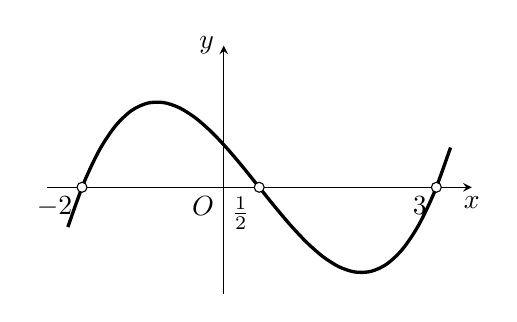
\begin{tikzpicture}[>=stealth,scale=.9]
\draw[->](-2.5,0)--(3.5,0)node[below]{$x$};
\draw[->](0,-1.5)--(0,2)node[left]{$y$};
\draw[domain=-2.2:3.2, smooth, very thick]plot(\x, {0.1*(\x+2)*(\x-3)*(2*\x-1)});
\foreach \x in {-2,3}
{
    \draw[fill=white](\x, 0)circle (2pt)node[below left]{$\x$};
}
\draw[fill=white](.5, 0)circle (2pt)node[below left]{$\frac{1}{2}$};
\node[below left]{$O$};
\end{tikzpicture}
\caption{}
\end{minipage}    \hfill
\begin{minipage}{.5\textwidth}
    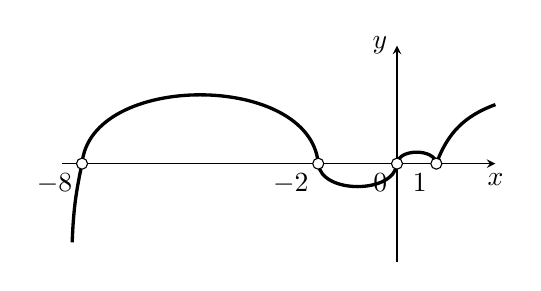
\begin{tikzpicture}[>=stealth, scale=.5]
\draw[->](-8.5,0)--(2.5,0)node[below]{$x$};
\draw[->](0,-2.5)--(0,3)node[left]{$y$};

\draw[very thick](-8.25,-2)[bend left=5] to (-8,0)[bend left=85]to (-2,0)[bend left=-85] to (0,0)[bend left=85] to (1,0)[bend left=25] to (2.5,1.5);
\foreach \x in {-2,0,1,-8}
{
    \draw[fill=white](\x, 0)circle (4pt)node[below left]{$\x$};
}
    \end{tikzpicture}
    \caption{}
    \end{minipage}    
\end{figure}

\begin{example}
解不等式$\frac{4}{x-1}\le x-1$.
\end{example}

\begin{solution}
\[\begin{split}
    \text{原不等式}&\Longleftrightarrow \frac{4}{x-1}-(x-1)\le 0 \Longleftrightarrow \frac{4-(x-1)^2}{x-1}\le 0\\
    &\Longleftrightarrow \frac{(3-x)(x+1)}{x-1}\le 0 \Longleftrightarrow \frac{(x-3)(x+1)}{x-1}\ge 0\\
    &\Longleftrightarrow \begin{cases}
        (x-3)(x+1)(x-1)\ge 0\\
        x-1\ne 0
    \end{cases}
\end{split}\]

$\therefore\quad $原不等式的解集是$[-1,0)\cup[3,+\infty)$. (图4.13)
\end{solution}

\begin{figure}[htp]
    \centering
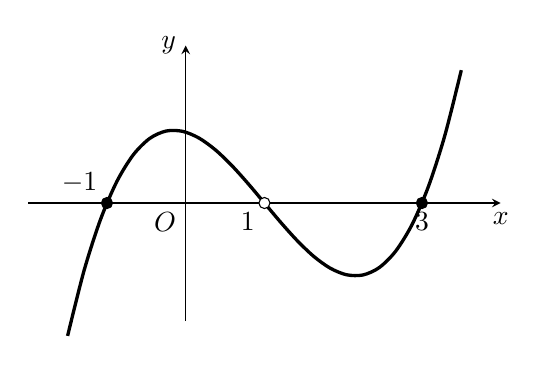
\begin{tikzpicture}[>=stealth]
    \draw[->](-2,0)--(4,0)node[below]{$x$};
    \draw[->](0,-1.5)--(0,2)node[left]{$y$};
    \draw[domain=-1.5:3.5, smooth, very thick]plot(\x, {0.3*(\x+1)*(\x-3)*(\x-1)});
    \foreach \x in {-1,3}
    {
        \draw[fill](\x, 0)circle (2pt);
    }
    \draw[fill=white](1, 0)circle (2pt)node[below left]{1};
    \node at (-1,0)[above left]{$-1$};
    \node at (3,0)[below]{$3$};
\node [below left]{$O$};
\end{tikzpicture}
    \caption{}
\end{figure}

\begin{example}
    解不等式$3x+5+\frac{1}{x-4}>2x+\frac{1}{x-4}+3$.
\end{example}

\begin{analyze}
    先消去不等号两边的分式将使解法简化,但消去后的不等式与原不等式不同解,这一点必须特别注意.
\end{analyze}

\begin{solution}
\[\text{原不等式}\Longleftrightarrow \begin{cases}
    3x+5>2x+3\\ x-4\ne 0
\end{cases} \Longleftrightarrow \begin{cases}
    x>-2\\ x\ne 4
\end{cases}\]

$\therefore\quad $原不等式的解集为$(-2,4)\cup (4,+\infty)$.
\end{solution}

\begin{example}
    解不等式$\frac{x-a}{(x+2)(x-3)}<0$\hfill (1)
\end{example}

\begin{solution}
\begin{equation}
    (1)\Longleftrightarrow (x-a)(x+2)(x-3)<0 \tag{2}
\end{equation}

由于$a$的不同取值使方程$(x-a)(x+2)(x-3)=0$的根在$x$轴上的相对位置不确定,故应对字母$a$的取值进行讨论。

\begin{figure}[htp]
    \centering
\begin{minipage}{.45\textwidth}
\begin{tikzpicture}[>=stealth, scale=.75]
\draw[->](-2.5,0)--(5.5,0)node[below]{$x$};
\draw[->](0,-1.5)--(0,3)node[left]{$y$};

\draw(-2.5,-1)[bend left=20] to (-2,0) [bend left=60] to (3,0)[bend right=30] to (4,0)[bend right=20] to (4.8,1.5);


\foreach \x in {-2,3}
{
    \draw[fill=white](\x, 0)circle (2pt)node[below]{$\x$};
}
\draw[fill=white](4, 0)circle (2pt)node[below]{$a$};
\node[below right]{$O$};
\end{tikzpicture}
\caption{}
\end{minipage}    \hfill
\begin{minipage}{.45\textwidth}
    \begin{tikzpicture}[>=stealth, scale=.75]
\draw[->](-2.5,0)--(5.5,0)node[below]{$x$};
\draw[->](0,-1.5)--(0,3)node[left]{$y$};

\draw(-2.5,-1)[bend left=20] to (-2,0) [bend left=60] to (3,0)[bend right=-30] to (4.8,1.5);


\foreach \x in {-2,3}
{
    \draw[fill=white](\x, 0)circle (2pt)node[below]{$\x$};
}
\node[below right]{$O$};
    \end{tikzpicture}
    \caption{}
    \end{minipage}    
\end{figure}


\begin{enumerate}[(i)]
    \item 当$a>3$时(图4.14),解集为$(-\infty,-2)\cup (3,a)$
    \item 当$a=3$时(图4.15),(2)变成$(x-3)^2(x+2)<0$
    
    $\therefore\quad $解集为$(-\infty,-2)$.
    \item 当$-2<a<3$时(图4.16),解集为$(-\infty,-2)\cup (a,3)$
    \item 当$a=-2$时(图4.17),(2)变成$(x+2)^2(x-3)<0$,解集为$(-\infty,-2)\cup (-2,3)$

\begin{figure}[htp]
    \centering
\begin{minipage}{.45\textwidth}
\begin{tikzpicture}[>=stealth, scale=.75]
\draw[->](-2.5,0)--(4.5,0)node[below]{$x$};
\draw[->](0,-1.5)--(0,3)node[left]{$y$};

\draw(-2.5,-1)[bend left=20] to (-2,0) [bend left=60] to (2,0)[bend right=30] to (3,0)[bend right=20] to (3.8,1);


\foreach \x in {-2,3}
{
    \draw[fill=white](\x, 0)circle (2pt)node[below]{$\x$};
}
\draw[fill=white](2, 0)circle (2pt)node[below]{$a$};
\node[below right]{$O$};
\end{tikzpicture}
\caption{}
\end{minipage}    \hfill
\begin{minipage}{.45\textwidth}
    \begin{tikzpicture}[>=stealth, scale=.75]
\draw[->](-3,0)--(5,0)node[below]{$x$};
\draw[->](0,-2.5)--(0,2)node[left]{$y$};

\draw(-2.75,-.75)[bend left=-20] to (-2,0) [bend right=60] to (3,0)[bend right=10] to (4.5,1.5);


\foreach \x in {-2,3}
{
    \draw[fill=white](\x, 0)circle (2pt);
}
\node[below left]{$O$};
\node at (-2,0)[above]{$-2$};
\node at (3,0)[below]{$3$};


    \end{tikzpicture}
    \caption{}
    \end{minipage}    
\end{figure}
    \item 当$a<-2$时(图4.18),解集为$(-\infty,a)\cup (-2,3)$
\end{enumerate}

\begin{figure}[htp]
    \centering
\begin{tikzpicture}[>=stealth, scale=.8]
\draw[->](-6,0)--(4.5,0)node[below]{$x$};
\draw[->](0,-2)--(0,1.5)node[left]{$y$};

\draw(-5.5,-1)[bend left=20] to (-5,0) [bend left=50] to (-2,0)[bend right=50] to  (3,0)[bend left=-20] to (3.5,1);

\draw[fill=white](-2, 0)circle (2pt)node[below left]{$-2$};
\draw[fill=white](-5, 0)circle (2pt)node[below]{$a$};
\draw[fill=white](3, 0)circle (2pt)node[below]{$3$};
\node[above right]{$O$};
\end{tikzpicture}
    \caption{}
\end{figure}

\end{solution}

\section*{习题十一}
\begin{center}
    \bfseries A
\end{center}

\begin{enumerate}
    \item 解下列不等式:
\begin{multicols}{2}
\begin{enumerate}[(1)]
    \item $3x-2+\frac{1}{5-x}>2x+1-\frac{1}{x-5}$
    \item $\frac{2x-3}{3x-4}<2$
    \item $\frac{x(x-3)}{x^2-3x+2}<0$
    \item $\frac{x^2}{x^2-6x+8}\ge 1$
    \item $\frac{x+1}{(x-2)^2 (x+1)}<1$
    \item $2+\frac{2}{x-1}\le \frac{5}{4-x}$
\end{enumerate}
\end{multicols}

\item (选择题)下列不等式中,与$\frac{x-3}{2-x}\ge 0$同解的是(\qquad )
\begin{multicols}{2}
\begin{enumerate}[(A)]
    \item $(x-3)(2-x)\ge 0$
    \item $(x-3)(2-x)>0$
    \item $\frac{2-x}{x-3}\ge 0$
    \item $\lg(x-2)\le 0$
\end{enumerate}
\end{multicols}
\end{enumerate}

\begin{center}
    \bfseries C
\end{center}
\begin{enumerate}
 \setcounter{enumi}{2}   
 \item 解关于$x$的不等式$5^{\tfrac{a(1-x)}{x-2}+1}<1$
\end{enumerate}

\section{无理不等式的解法}
在根号内含有未知数的不等式称为\textbf{无理不等式}。如$\sqrt{x-1}>x-3$, $\sqrt{x}+2<\sqrt{2x-1}+1$等.

解无理不等式应注意:
\begin{enumerate}[(1)]
\item 必须使出现在不等式中的根式有意义,这就需要求出根式中函数的定义域;
\item 无理不等式的求解,根本是\textbf{化归}为有理不等式,转化的依据是4.10节中的定理5。
\end{enumerate}

以下研究几个例子。

\begin{example}
解不等式$\sqrt{x-1}>x-3$\hfill (1)
\end{example}

\begin{analyze}
\begin{enumerate}
    \item 为使用定理5,应对有理式$x-3$进行讨论。
    \item (1)式的结构特征使我们想到换元法。
    \item (1)式两边都是我们熟知的函数。
\end{enumerate}
\end{analyze}


\begin{solution}
\textbf{解法1:}
\[(1)\Longleftrightarrow {\rm (I)}\begin{cases}
    x-3\ge 0& \text{(限制条件)}\\
x-1\ge 0 &\text{(定义域)}\\
x-1>(x-3)^2
\end{cases} \text{和}\quad {\rm (II)}\begin{cases}
    x-3<0& \text{(限制条件)}\\
    x-1\ge 0 &\text{(定义域)}\\
\end{cases}\]
而
\[{\rm (I)}\Longleftrightarrow \begin{cases}
    x\ge 3\\
    x-1>(x-3)^2
\end{cases}\Longleftrightarrow \begin{cases}
    x\ge 3\\
    (x-2)(x-5)<0
\end{cases}\]
$\therefore\quad 3\le x<5$.

\[{\rm (II)}\Longleftrightarrow \begin{cases}
    x< 3\\
    x\ge 1
\end{cases}\qquad \therefore\quad 1\le x<3\]

$\therefore\quad $(1)的解集为$[3,5)\cup[1,3)$,即$[1,5)$.

\textbf{解法2:}
(1)即$\sqrt{x-1}>(x-1)-2$.

令$t=\sqrt{x-1}\ge 0$,得$\begin{cases}
    t\ge 0\\t^2-t-2<0
\end{cases}$

解之,得$0\le t<2$,即$0\le \sqrt{x-1}<2\Longleftrightarrow \begin{cases}
    x-1\ge 0\\ x-1<4
\end{cases}$

$\therefore\quad 1\le x<5$.

\textbf{解法3:}
令$y_1=\sqrt{x-1}$,$y_2=x-3$,从而(1)的解集就是使函数$y_1>y_2$的$x$的取值范围。在同一个坐标系中分别作出两个函数的图象(图4.19). 设它们交点的横坐标是$x_0$,则$\sqrt{x_0-1}=x_0-3>0$

解之,得$x_0=2$(舍)或$x_0=5$

$\therefore\quad $(1)的解集为$[1,5)$.

\begin{figure}[htp]
    \centering
\begin{tikzpicture}[>=stealth, scale=.8]
\draw[->](-1,0)--(7,0)node[below]{$x$} ;   
\draw[->](0,-4)--(0,4)node[left]{$y$} ;
\draw[domain=1:6, smooth, samples=100, very thick]plot(\x, {sqrt(\x-1)})node[right]{$y_1=\sqrt{x-1}$};
\draw[domain=-.5:6, smooth, very thick]plot(\x, {\x-3});
\node at (1.5,-2)[right]{$y_2=x-3$};
\foreach \x in {-3,-2,-1,1,2,3}
{
    \draw(0,\x)--(.1,\x);
}
\foreach \x in {1,3}
{
    \draw(\x,0)node[below]{\x}--(\x,.1);
}
\draw[dashed](5,0)node[below]{$x_0$}--(5,2);
\node [below left]{$O$};

\draw[fill](1,0) circle (2pt);

\end{tikzpicture}
    \caption{}
\end{figure}

\end{solution}

\begin{rmk}
解法1是通法,应熟练掌握。换元法与图象法的突破口是认清式子的结构特征。
\end{rmk}

\begin{example}
解不等式$(x-1)\sqrt{x+2}\ge 0$\hfill (1)
\end{example}

\begin{solution}
\[(1)\Longleftrightarrow \begin{cases}
    (x-1)\sqrt{x+2}>0& (2)\\
    (x-1)\sqrt{x+2}=0 & (3)
\end{cases}\]
\[(2)\Longleftrightarrow \begin{cases}
    x+2\ge 0\\ x-1>0 
\end{cases}\qquad \therefore\quad x>1\]
(3)的解集是$x=1$或$x=-2$.

$\therefore\quad $(1)的解集为$[1,+\infty)\cup\{-2\}$.
\end{solution}

\begin{example}
解不等式$\sqrt{2ax-a^2}>a-x\; (a>0)$\hfill (1)
\end{example}

\begin{solution}
\[(1)\Longleftrightarrow {\rm (I)}\begin{cases}
    a-x\ge 0\\
    2ax-a^2\ge 0\\
    2ax-a^2>(a-x)^2
\end{cases}\text{和}\quad {\rm (II)}\begin{cases}
    a-x<0\\ 2ax-a^2\ge 0
\end{cases}\]
而
\[\begin{split}
{\rm (I)}&\Longleftrightarrow \begin{cases}
    a-x\ge 0\\ 2ax-a^2>(a-x)^2
\end{cases}\Longleftrightarrow \begin{cases}
    x\le a\\(x-2a)^2<2a^2
\end{cases}\\
&\Longleftrightarrow \begin{cases}
    x\le a\\|x-2a|<\sqrt{2}a
\end{cases}\Longleftrightarrow \begin{cases}
    x\le a\\ 2a-\sqrt{2}a<x\le 2a+\sqrt{2}a
\end{cases}
\end{split}\]
$\therefore\quad 2a-\sqrt{2}a<x\le a\quad (\because\quad a>0)$

\[{\rm (II)}\Longleftrightarrow \begin{cases}
    x>a\\ x\ge \frac{a}{2}
\end{cases}\qquad \therefore\quad x>a\quad (\because \quad a>0)\]
$\therefore\quad $(1)的解集是$(2a-\sqrt{2}a,a]\cup (a,+\infty)=\left((2-\sqrt{2})a,+\infty\right)$
\end{solution}


\section*{习题十二}
\begin{center}
    \bfseries A
\end{center}
解下列不等式(1—8题)
\begin{enumerate}
    \item $4x-3+\sqrt{10-x}>3x+2+\sqrt{10-x}$
    \item $\sqrt{3-x}>x-2$
    \item $\sqrt{2x^{2}-6x+4}<x+2$
    \item $\sqrt{3x-15}-\sqrt{x-4}\ge 0$
    \item $\sqrt{4-\log_{0.3}x}<\log_{0.3}x-2$ (提示:令$\log_{0.3}x=y$)
    \item $\sqrt{x-2}-\sqrt{x-5}>1$
\end{enumerate}


\begin{center}
    \bfseries B
\end{center}

\begin{enumerate}\setcounter{enumi}{6}
    \item $\sqrt{\log_{2}^{2}x+\log_{2}x-2}> 2\log_{2}x-2$
    \item $(x-1)\sqrt{x^{2}-x-2}\ge 0$
    \item 设$A= \{ x\mid 5- x> \sqrt {2(x- 1) }\}$, 
$B=\left\{x\mid x^{2}-ax\le x-a\right\}$,
要使$A\subset B$, 求实数$a$的取值范围。
\item 解关于$x$的不等式$\sqrt{2x-a}<\sqrt{x+1}$
\end{enumerate}


\begin{center}
    \bfseries C
\end{center}

\begin{enumerate}\setcounter{enumi}{10}
    \item 解关于$x$的不等式$\sqrt{a-2x}>a-x$(提示:参考例1的解法2).
\end{enumerate}

\section{绝对值不等式的性质、解法与证明}

在绝对值符号中含有未知数的不等式称为\textbf{绝对值不等式}。如
$|x-2|<3$, $|x-1|-|x+2|\ge 5$等。

\begin{thm}{实数绝对值的定义}
若$a\in\R$,那么
\[|a|=\begin{cases}
    a, &a>0\\
    0, &a=0\\
    -a, &a<0\\
\end{cases}\]
显然有$$-|a|\le a\le |a|$$
\end{thm}

\begin{thm}
    {最简绝对值不等式的解集(填空)}
\begin{enumerate}[(1)]
\item 若$|x|<R$,则$x\in \blank$;
\item 若$|x|>r,\; (r>0)$,则$x\in\blank$;
\item 若$r<|x|<R,\; (0<r<R)$,则$x\in\blank$.
\end{enumerate}
\end{thm}

\begin{note}
\begin{enumerate}[(i)]
    \item 若把$x$看作数轴上点$P$的坐标,则$|x|$就是点$P$到原点$O$的距离。那么,上述三个最简绝对值不等式的解集的几何意义十分明显。
    \item 把三个最简绝对值不等式写成与它等价的解集的形式是脱去绝对值符号的重要方法,应该熟练掌握。
    \item 为了“脱去”绝对值号,有时也采用不等式两边分别平方的办法。如
\[|A|\ge |B|\Longleftrightarrow A^2\ge B^2\]
(这是因为$|A|\ge |B|\ge 0$)
\item 这里的正数$R$、$r$不仅可以放宽到零和负数,而且进一步还可以放宽为含未知数的解析式(这无疑会给解题带来极大的方便):
\begin{itemize}
    \item 推广1:$|x|<\varphi(x)\Longleftrightarrow -\varphi(x)<x<\varphi(x)$;
    \item 推广2:$|x|>\varphi(x)\Longleftrightarrow x<-\varphi(x)\text{或}x>\varphi(x)$.
\end{itemize}
(用5.11中定理1的证法可以证明这两个推广)
\end{enumerate}
\end{note}

\begin{example}
解不等式$|x^2+3x-8|\le 10$\hfill (1)
\end{example}

\begin{solution}
    $(1)\Longleftrightarrow -10\le x^2+3x-8\le 10 $\hfill (2)
\[\begin{split}
  (2) & \Longleftrightarrow \begin{cases}
        -10\le x^2+3x-8\\
        x^2+3x-8\le 10
    \end{cases}
     \Longleftrightarrow \begin{cases}
        x^2+3x+2\ge 0\\
        x^2+3x-18\le 0
    \end{cases}\\
    &\Longleftrightarrow \begin{cases}
        (x+2)(x+1)\ge 0,&(3)\\
        (x+6)(x-3)\le 0,&(4)
    \end{cases}
\end{split}\]

很清楚(图4.20), 不等式组(3)、(4)的解集为$[-6,-2]\cup [-1,3]$.
\end{solution}

\begin{figure}[htp]
    \centering
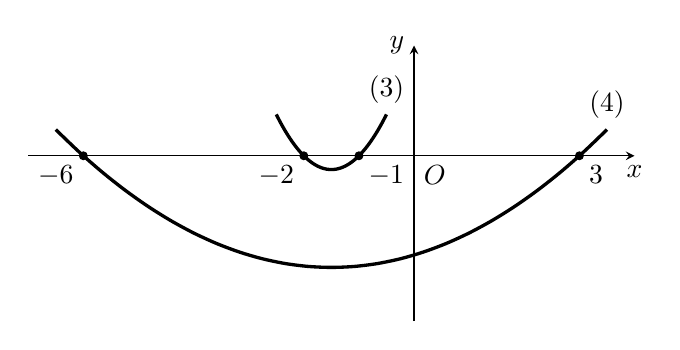
\begin{tikzpicture}[>=stealth, scale=.7]
\draw[->](-7,0)--(4,0)node[below]{$x$} ;   
\draw[->](0,-3)--(0,2)node[left]{$y$} ;
\draw[domain=-2.5:-.5, smooth, very thick]plot(\x, {(\x+2)*(\x+1)})node[above]{$(3)$};
\draw[domain=-6.5:3.5, smooth, very thick]plot(\x, {0.1*(\x+6)*(\x-3)})node[above]{$(4)$};
\foreach \x in {-6,-2}
{
    \node at (\x,0)[below left]{$\x$};
    \draw[fill](\x,0) circle(2pt);
}
\foreach \x in {-1,3}
{
    \node at (\x,0)[below right]{$\x$};
    \draw[fill](\x,0) circle(2pt);
}
\node[below right]{$O$};
\end{tikzpicture}
    \caption{}
\end{figure}

\begin{example}
    解不等式$|5x-x^2|>6$\hfill (1)
\end{example}

\begin{solution}
(1)即 $|x^2-5x|>6$\hfill (*)

(习惯上,我们总是先按x的降幂排列,并使x的最高次项的系数为正)。

\[\begin{split}
    (*)&\Longleftrightarrow x^2-5x<-6,\text{或}x^2-5x>6 \\
    &\Longleftrightarrow x^2-5x+6<0,\text{或}x^2-5x-6>0\Longleftrightarrow \begin{cases}
        (x-2)(x-3)<0,& (2)\\
        (x-6)(x+1)>0,& (3)
    \end{cases}
\end{split} \]
(2)的解集是$(2,3)$;(3)的解集是$(-\infty,-1)\cup (6,+\infty)$.

$\therefore\quad (1)$的解集为$(2,3)\cup (-\infty,-1)\cup (6,+\infty)$
\end{solution}

\begin{example}
    解不等式$3\le |5-2x|<9$\hfill (1)
\end{example}

\begin{solution}
先把(1)改写成 $3\le |2x-5|<9$\hfill (*)

根据最简绝对值不等式(3),有
\[(*)\Longleftrightarrow \begin{cases}
    -9< 2x-5\le -3,& (2)\\
    3\le 2x-5<9,&(3)
\end{cases}\]

$\therefore\quad (1)$的解集为$(-2,1]\cup[4,7)$.
\end{solution}

\begin{rmk}
上述三例,都是利用最简绝对值不等式的解集脱去了绝对值符号,这是最常用也是最基本的方法。若要用“先平方”的办法脱去绝对值号,运算量一般都较大,而且有时还有可能增解,这时必须检验。
\end{rmk}

\begin{example}
    解不等式$\left|x^2-4\right|\le  x+2$\hfill (1)
\end{example}

\begin{solution}
    根据推广1,$(1)\Longleftrightarrow-x-2\le  x^{2}-4\le  x+2$
即
\[\begin{cases}x^{2}-4\geqslant-x-2,\\
    x^{2}-4\leqslant x+2,
\end{cases}\Longleftrightarrow
\begin{cases}
    x^{2}+x-2\geqslant0,\\
    x^{2}-x-6\leqslant0,
\end{cases}\Longleftrightarrow\begin{cases}(x+2)(x-1)\geqslant0,\\
    (x+2)(x-3)\leqslant0.
\end{cases}\]
$\therefore\quad $ (1)的解集为$[1,3]\cup \{-2\}$.
\end{solution}

\begin{thm}{思考题}
    用图象法解此题行吗?试一试。
\end{thm}

\begin{example}
    解不等式$\left|\frac{x+3}{2x-1}\right|\leqslant1$
\end{example}

\begin{solution}
\textbf{解法1:}原不等式同解于:
\[\begin{split}
    &|x+3|\leqslant|2x-1|, \text{ 且 } 2x-1\neq0,\\
&\Longleftrightarrow (x+3)^{2}\leqslant(2x-1)^{2}\text{ 且 }2x-1\neq0,\\
&\Longleftrightarrow 3x^{2}-10x-8\geqslant 0\text{ 且 }2x-1\neq0\\
&\Longleftrightarrow(3x+2)(x-4)\geqslant0\text{ 且 }2x-1\neq0.
\end{split}\]

$\therefore\quad $(1)的解集为$\left(-\infty,-\frac23\right]\cup[4,+\infty)$.    

\textbf{解法2:}
\[\begin{split}
    (1)&\Longleftrightarrow \left(\frac{x+3}{2x-1}\right)^2-1\le 0\\
    &\Longleftrightarrow \frac{3x^2-10x-8}{(2x-1)^2}\ge 0 \Longleftrightarrow \begin{cases}
        (3x+2)(x-4)\ge 0\\
        (2x-1)^2\ne 0
    \end{cases}
\end{split} \]
$\therefore\quad $(1)的解集为$\left(-\infty,-\frac{2}{3}\right]\cup [4,+\infty)$.
\end{solution}

\begin{example}
    解不等式$|x+7|-|x-2|<3$\hfill (1)
\end{example}

\begin{analyze}
这里出现了两个绝对值号,上述三个最简绝对值不等式的结果已不能使用,只好根据“实数绝对值的定义”去脱绝对值号。为此,需要分别求出$|x+7|$与$|x-2|$的零点(使函数值为零的$x$值),再以诸零点为边界,把$(-\infty,+\infty)$分成几个相互连接的区间,然后在每个区间上去探求(1)的解。也就是说,把在实数集$\R$上解不等式(1),转化成在
$\R$的子区间上分别去解(1)。这就是此法的实质。

\end{analyze}

\begin{solution}
    由于$-7$, 2分别是$|x+7|$与$|x-2|$的零点,它们把区间$(-\infty,+\infty)$分成三个子区间(图4.21)。

\begin{figure}[htp]
    \centering
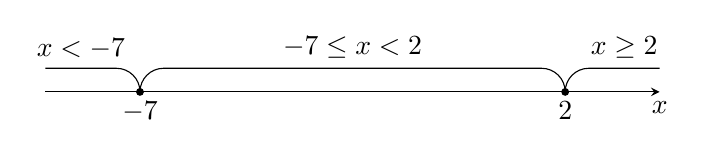
\begin{tikzpicture}[>=stealth, scale=.6]
    \draw[->](-9,0)--(4,0)node[below]{$x$};
\foreach \x in {-7,2}
{
    \node at (\x,0)[below]{$\x$};
    \draw[fill](\x,0) circle(2pt);
}    
\draw(-9,.5)--node[above]{$x<-7$}(-7.5,.5)[bend left=45] to (-7,0);
\draw(2,0)[bend left=-45] to (2-.5,.5)--node[above]{$-7\le x<2$}(-6.5,.5)[bend left=-45] to (-7,0);
\draw(4,.5)--node[above]{$x\ge 2$}(2.5,.5) [bend left=-45] to (2,0);
\end{tikzpicture}
    \caption{}
\end{figure}

由此,(1)可化成三个不等式组:
\begin{enumerate}[(1)]
    \item $\begin{cases}x\geqslant2,\\(x+7)-(x-2)<3,\end{cases}\Longleftrightarrow\begin{cases}x\geqslant2,\\9<3.\end{cases}$
    
    $\therefore\quad$ 解集$X_1=\emptyset$

    \item $\begin{cases} - 7\leq x< 2, \\ ( x+ 7) + ( x- 2) < 3, \end{cases} \Longleftrightarrow \begin{cases} - 7\leq x< 2, \\ x< - 1.  \end{cases}$
    
    $\therefore\quad$ 解集$X_2=[-7,-1)$
    
\item $\begin{cases} x< - 7, \\ - ( x+ 7) - [ - ( x- 2) ] < 3. 
\end{cases} 
\Longleftrightarrow \begin{cases} x< - 7, \\ - 9< 3. \end{cases}$

$\therefore\quad$ 解集$X_3=(-\infty,-7)$.
\end{enumerate}

$\therefore\quad$(1)的解集为$X_1\cup X_2\cup X_3=(-\infty,-1)$.
\end{solution}

\begin{thm}{思考题}
\begin{enumerate}[(1)]
    \item 根据(1)式的几何意义,你能通过画出数轴直接看出它的解集吗?
    \item 根据几何意义,你能判断不等式$|x|+|x-3|<1$无解吗?
\end{enumerate}
\end{thm}

\begin{example}
    解不等式$\frac{\log_{0.1}|x-2|}{x^2-4x}<0$\hfill (1)
\end{example}

\begin{solution}
\[\begin{split}
    (1)&\Longleftrightarrow \begin{cases}
        \log_{0.1}|x-2|>0\\
        x^2-4x<0
    \end{cases}\text{或}\quad \begin{cases}
        \log_{0.1}|x-2|<0\\
        x^2-4x>0
    \end{cases}\\
    &\Longleftrightarrow \begin{cases}
        0<|x-2|<1\\
        x(x-4)<0
    \end{cases}\text{(图4.22)\quad 或}\quad \begin{cases}
        |x-2|>1 \\
        x(x-4)>0
    \end{cases}\text{(图4.23)}\\
\end{split}\]

\begin{figure}[htp]
    \centering
\begin{minipage}{.45\textwidth}
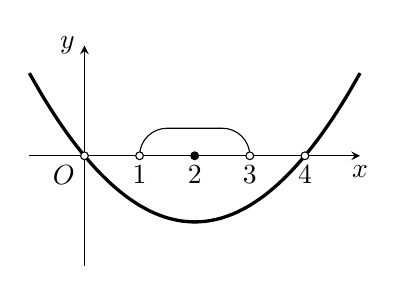
\begin{tikzpicture}[>=stealth, scale=.7]
\draw[->](-1,0)--(5,0)node[below]{$x$};
\draw[->](0,-2)--(0,2)node[left]{$y$};
\node[below left]{$O$};
\foreach \x in {1,2,3,4}
{
    \node at (\x,0)[below]{$\x$};
}
\draw(1,0)[bend left=45] to (1.5,.5)--(3-.5,.5)[bend left=45] to (3,0);
\draw[domain=-1:5, smooth, very thick]plot(\x, {0.3*\x*(\x-4)});

\foreach \x in {0,1,3,4}
{
    \draw[fill=white](\x,0)circle (2pt);
}
\draw[fill](2,0)circle (2pt);


\end{tikzpicture}
\caption{}
\end{minipage}
\hfill
\begin{minipage}{.45\textwidth}
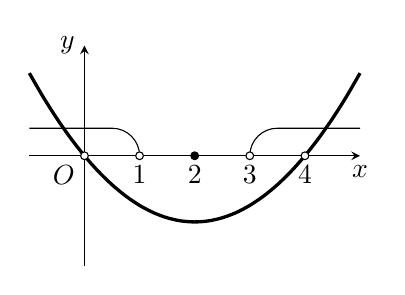
\begin{tikzpicture}[>=stealth, scale=.7]
    \draw[->](-1,0)--(5,0)node[below]{$x$};
    \draw[->](0,-2)--(0,2)node[left]{$y$};
    \node[below left]{$O$};
    \foreach \x in {1,2,3,4}
{
    \node at (\x,0)[below]{$\x$};
}
\draw(3,0)[bend left=45] to (3.5,.5)--(5,.5);
\draw(-1,.5)--(.5,.5)[bend left=45] to (1,0);
\draw[domain=-1:5, smooth, very thick]plot(\x, {0.3*\x*(\x-4)});

\foreach \x in {0,1,3,4}
{
    \draw[fill=white](\x,0)circle (2pt);
}
\draw[fill](2,0)circle (2pt);
\end{tikzpicture}
\caption{}
\end{minipage}
\end{figure}

$\therefore\quad $(1)的解集为$(1,2)\cup (2,3)\cup (-\infty,0)\cup (4,+\infty)$.

\end{solution}

\begin{example}
    用简捷方法解$|x^2-2|<|x|$ \hfill (1)
\end{example}

\begin{solution}
\textbf{解法1:}(1)即$\Big||x|^2-2\Big|<|x|$

令$|x|=y$,则上式$\Longleftrightarrow |y^2-2|<y\Longleftrightarrow 1<y<2$

$\therefore\quad 1<|x|<2$.

从而(1)的解集为$(-2,-1)\cup (1,2)$.

\textbf{解法2:} $\because\quad $不等号两边的函数都为偶函数,

$\therefore\quad $若$x$为(1)的解,则$-x$也为(1)的解。

当$x\ge 0$时,$(1)\Longleftrightarrow |x^2-2|<x$,
解之得$1<x<2$

$\therefore\quad $当$a\le 0$时,必有$-2<x<-1$, 
从而,(1)的解集为$(-2,-1)\cup (1,2)$.
\end{solution}

\section*{习题十三}
\begin{center}
    \bfseries A
\end{center}

\begin{enumerate}
    \item 解不等式:
\begin{multicols}{2}
\begin{enumerate}[(1)]
    \item $|x+1|<\sqrt{2}$
    \item $1<|x-4|\leqslant2$
    \item $| x^{2}-2x-3|-2>0$
    \item $3\leqslant|5-2x|<9$
    \item $|x^{2}+2x-1|<2$
    \item $|x^{2}-1|\geqslant x$
    \item $|x^{3}-1|>1-x$
\end{enumerate}
\end{multicols}

\item 解不等式:
\begin{multicols}{2}
\begin{enumerate}[(1)]
    \item $|x+6|-|3-2x|>4$
    \item $\sqrt{4-4x+x^{2}}+|x-3|-1\leq0$
    \item $\sqrt{x^{2}+2x+1}-2|2-x|>5-x$
    \item $|x|+|x-3|\leqslant1$
\end{enumerate}
\end{multicols}

\item 求$|x-a|+|x-b|+|x-c|$的最小值。(提示:从几何意义上考虑最简便)

\item 解不等式:
\begin{multicols}{2}
\begin{enumerate}[(1)]
    \item $\left|\frac{x-3}{x+1}\right|\ge 1$
    \item $\left|\frac{2x-1}{2-x}\right|<2$
\end{enumerate}
\end{multicols}

\item 用最简捷的方法解下列不等式:
\begin{multicols}{3}
\begin{enumerate}[(1)]
    \item $\left|\frac{1}{x}\right|<\frac{1}{2}$
    \item $\left|\frac{1}{x}\right|\ge \frac{1}{3}$
    \item    $1\le \left|\frac{1}{x-2}\right|\le 2$
    \item $0\le \frac{1}{x+1}\le 2$
    \item $2<\frac{1}{x+1}\le 3$
\end{enumerate}
\end{multicols}
\end{enumerate}


\begin{center}
\bfseries B
\end{center}

\begin{enumerate}
\setcounter{enumi}{5}    
\item 用最简捷的方法解不等式
$x^2-3x-4>0$.
\item 若不等式$|x|+|x-3|<a$
有解,求实数$a$的取值范围。
\item 解不等式(复习指数与对数不等式的解法):
\begin{enumerate}[(1)]
    \item $4^x-6^x-2.9^x>0$
    \item $a^{2x}+1<a^{x+2}+a^{x-2}$ ($a>0$且$a\ne 1$)
    \item $\log_{\tfrac{1}{2}}(x+1)+\log_{\tfrac{1}{2}}(x+4)<1$
    \item $\log_2(x+1)+\log_{0.25}(x-1)>\log_4(2x-1)$
    \item $\log_x(x+2)>2$
    \item $\log_2 x-\log_{\sqrt{x}}2<1$
\end{enumerate}


\item 用换元法解不等式:
\begin{enumerate}[(1)]
    \item $\log_3 x+10\log_x 27 >4$
    \item $\log_a x>6\log_x a-1$ ($a>0$且$a\ne 1$)
    \item $\frac{1}{1+\lg x}+\frac{1}{1-\lg x}>2$
    \item $x^{\log_a x}>\frac{x^4\cdot \sqrt{x}}{a^2}$ ($a>0$且$a\ne 1$)
    \item $\left|\log_{\sqrt{a}x}-2\right|-\left|\log_a x-2\right|<2$
\end{enumerate}

\item 若集合$A=\left\{n\left|-\frac{1}{2}\le \log_{\tfrac{1}{n}}2\le -\frac{1}{3},\; n\in\Z \right. \right\}$,试求$A$的元素的个数和子集的个数。
\end{enumerate}

\begin{center}
    \bfseries C
\end{center}
\begin{enumerate}
  \setcounter{enumi}{10}  
  \item  解关于$x$的不等式$|x|>\frac{6a^2}{a-x}$
  \item 解不等式$\frac{\lg 2x}{\lg(4x-5)}<2$
  \item 解不等式$|\sqrt{2x-1}-x|<2$
  \item 当$a>1$时,解关于$x$的不等式$|a^x-1|+|a^{2x}-3|>2$
\end{enumerate}


\subsection{实数的绝对值的运算性质}
根据实数绝对值的定义,可以得到:

\begin{thm}
    {性质1}
$$|ab|=|a|\cdot |b|\qquad (\forall a,b\in\R)$$
\end{thm}

\begin{thm}
  {性质2}
$$\left|\frac{a}{b}\right|=\frac{|a|}{|b|}\qquad (\forall a,b\in\R, \text{ 且 }b\ne 0)$$
\end{thm}
(你能给出这两个性质的证明吗?)  


\begin{thm}
    {性质3} 对于任意的实数$a,b$,
\begin{enumerate}[(1)]
    \item $|a+b|\le |a|+|b|$,等号当且仅当$ab\ge 0$时成立;
\item  $|a+b|\ge |a|+|b|$,等号当且仅当$ab\le 0$时成立.
\end{enumerate}
\end{thm}

\begin{proof}
    欲证(1),只要证 $(|a+b|)^2\le (|a|+|b|)^2$,即
\[a^2+2ab+b^2\le a^2+b^2+2|ab|\]
很明显,此式当$ab<0$时“$<$”成立,当
$ab\ge 0$时“$=$”成立。

(2)的证明是类似的。
\end{proof}

\begin{thm}
    {性质4} 对于任意实数
$a,b$, 
\begin{enumerate}[(1)]
    \item $|a-b|\le |a|+|b|$,等号当且仅当$ab\le 0$时成立;
\item  $|a-b|\ge \Big||a|-|b|\Big|$,等号当且仅当$ab\ge 0$时成立.
\end{enumerate}
\end{thm}

\begin{proof}
    在性质3中以$(-b)$代替$b$即可。

    上述两个性质,也可以统一写成
\[ \Big||a|-|b|\Big|\le |a\pm b|\le |a|+|b| \]
\end{proof}

\begin{example}
    已知$|x|<\frac{a}{4}$, $|y|<\frac{a}{6}$,求证:$|2x-3y|<a$.
\end{example}

\begin{proof}
$\because\quad |2x-3y|<|2x|+|3y| $,
而
\[\begin{split}
   | 2x|&=|2|\cdot |x|=2|x|<2\cdot \frac{a}{4}=\frac{a}{2}\\
    |3y|&=|3|\cdot |y|=3|y|<3\cdot \frac{a}{6}=\frac{a}{2}
\end{split}\]|
$\therefore\quad |2x-3y|<\frac{a}{2}+\frac{a}{2}=a$.


\end{proof}

\begin{example}
    解不等式$|x|+|x-3|<1$.
\end{example}
 
\begin{solution}
$\because\quad |x|+|x-3|\ge |x-(x-3)|=3$

$\therefore\quad $原不等式无解。
\end{solution}


\section*{习题十四}
\begin{center}
    \bfseries A
\end{center}
\begin{enumerate}
    \item  已 知 $| x- a| < \frac{\varepsilon}{2}$, $| y- b| <{\varepsilon}{2}$, 求证:
\begin{enumerate}[(1)]
    \item $|(x+y)-(a+b)|<\varepsilon$
    \item $|(x-y)-(a-b)|<\varepsilon$
\end{enumerate}

\item  已知$|x|<\sqrt a$, $|y|<\sqrt b$, 求证$|xy|<\sqrt{ab}.$
\item 已知$|x|<m\varepsilon$, $|y|>m>0$, $\varepsilon>0$. 
求证:$\left|\frac\pi y\right|<\varepsilon$
\item  已知$|a_n-\ell|<1$,求证$|a_n|<|\ell|+1.$

\item 已知$|x|<\frac\varepsilon3$, $|y|<\frac\varepsilon6$, $|z|<\frac\varepsilon9$, $\varepsilon>0$, 求证
$|x+2y-z|<\varepsilon$.
\end{enumerate}


\begin{center}
    \bfseries B
\end{center}

\begin{enumerate}\setcounter{enumi}{5}
    \item 判断下列命题的真假(应简述理由):
\begin{enumerate}[(1)]
    \item $|x-100|+|x+100|<5$,无解;
    \item $2|x-10|+|x-1|<2$,无解;
    \item $\sqrt{4-4x+x^2}+|x-3|-1\le 0$的解是$[2,3]$;
    \item $|x-5|+|2-x|\le -5$,无解;
    \item $|x-5|+|x+2|\le 6$,无解。
\end{enumerate}

\item 利用最简绝对值不等式的解集(1)证明本节性质3(1).
\item \begin{enumerate}[(1)]
    \item 求不等式$|x-3|+|x-5|<a$有解的充要条件;
    \item 求不等式$|x-3|-|x-5|\ge a$有解的充要条件。
\end{enumerate}
\end{enumerate}

\subsection{绝对值不等式的证明}
\begin{example}
    已知$|a|<1$, $|b|<1$, 
求证:$\left|\frac{a+b}{1+ab}\right|<1$\hfill (1)
\end{example}

\begin{proof}
\textbf{证法1:}欲证(1),只要证    
\begin{equation}
    -1<\frac{a+b}{1+ab}<1 \tag{2}
\end{equation}
欲证(2),只要证
\begin{equation}
-1<\frac{a+b}{1+ab}\quad \text{且}\quad \frac{a+b}{1+ab}<1  \tag{3}
\end{equation}
欲证(3),只要证
\begin{equation}
\frac{a+b}{1+ab}+1>0 \quad \text{且}\quad \frac{a+b}{1+ab}-1<0  \tag{4}
\end{equation}
但是
\[ \frac{a+b}{1+ab}+1 = \frac{a+b+1+ab}{1+ab}=\frac{(b+1)(a+1)}{1+ab}>0\]
($\because\quad |a|<1,\quad |b|<1\qquad \therefore\quad a+1>0,\quad b+1>0,\quad 1+ab>0$)

\[ \frac{a+b}{1+ab}-1 = \frac{a+b-1-ab}{1+ab}=\frac{-(1-a)(1-b)}{1+ab}<0\]
($\because\quad |a|<1,\quad |b|<1\qquad \therefore\quad 1-a>0,\quad 1-b>0,\quad 1+ab>0$)

$\therefore\quad $(4)成立,从而(1)成立.

\textbf{证法2:}我们利用$|A|\ge |B|\Longleftrightarrow A^2\ge B^2$来证(1)

欲证(1), 只要证
\begin{equation}
\left(\frac{a+b}{1+ab}\right)^2<1,\quad (1+ab)\ne 0\tag{2}
\end{equation}
欲证(2), 只要证
\begin{equation}
   (a+b)^2<(1+ab)^2,\quad 1+ab\ne 0  \tag{3} 
\end{equation}
欲证(3), 只要证
\begin{equation}
1-a^2-b^2+a^2b^2>0,\quad 1+ab\ne 0  \tag{4} 
\end{equation}
欲证(4), 只要证
\begin{equation}
(1-a^2)(1-b^2)>0,\quad 1+ab\ne 0  \tag{5} 
\end{equation}
而由$|a|<1$,$|b|<1$得知(5)成立,从而(1)成立。
\end{proof}

\begin{example}
求证 $\frac{|a+b|}{1+|a+b|}\le \frac{|a|}{1+|a|}+\frac{|b|}{1+|b|}$\hfill (1)
\end{example}

\begin{analyze}
    问题的困难在于三个分式的分母都不相同。当然
我们可以用分析法先去分母逆推之,直至发现明显不等式为
止,但这样做运算较繁。

在此,我们先把右边缩小化成同分母的式子。
\end{analyze}

\begin{proof}
$\because\quad \frac{|a|}{1+|a|}\ge \frac{|a|}{1+|a|+|b|},\quad \frac{|b|}{1+|b|}\ge \frac{|b|}{1+|a|+|b|}$

$\therefore\quad $欲证(1), 只要证
\begin{equation}
\frac{|a+b|}{1+|a+b|}\le \frac{|a|}{1+|a|+|b|}+\frac{|b|}{1+|a|+|b|}=\frac{|a|+|b|}{1+|a|+|b|} \tag{2}
\end{equation}
欲证(2), 只要证
\begin{equation}
    |a+b|\cdot (1+|a|+|b|)\le (1+|a+b|)(|a|+|b|)\tag{3}
\end{equation}
即
\[|a+b|\le |a|+|b|\]
此式显然成立$\Longrightarrow$(2)成立$\Longrightarrow$(1)成立。
\end{proof}

作为本节最后一例,介绍用几何方法证代数不等式。

\begin{example}
求证:$\sqrt{a^2+b^2}+\sqrt{a^2+(1-b)^2}+\sqrt{b^2+(1-a)^2}+\sqrt{(1-a)^2+(1-b)^2}\ge 2\sqrt{2}$
\end{example}

\begin{analyze}
    若把$A(a,b)$看作是坐标系$xOy$中的点,那么
$\sqrt{a^2+b^2}=|OA|$. 为了出现$\sqrt{2}$,可以取$B(1,1)$,则$\sqrt{2}=|OB|$,有了这两个点,$\sqrt{(1-a)^2+(1-b)^2}$可以表示成$|AB|$,类似地可以处理其余两个根式。
\end{analyze}

\begin{proof}

\noindent
\begin{minipage}{.45\textwidth}
    在坐标系$xOy$中(图4.24)取定三个点
$A(a,b)$,$B(1,1)$, $C(1-a,b)$.

显然
\[\begin{split}
|OA|&=\sqrt{a^2+b^2}\\
|AB|&=\sqrt{(1-a)^2+(1-b)^2}\\
|OC|&=\sqrt{(1-a)^2+b^2}\\
|CB|&=\sqrt{a^2+(b-1)^2}\\
|OB|&=\sqrt{2}\\
\end{split}\]
\end{minipage}
\begin{minipage}{.45\textwidth}
\centering
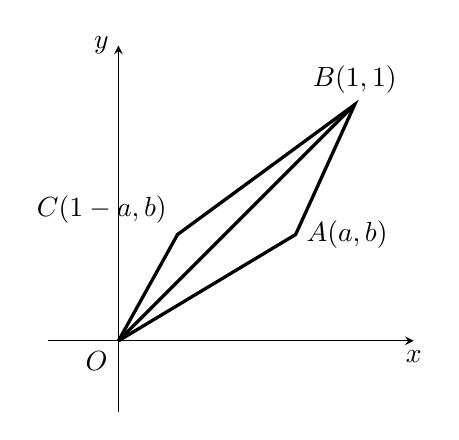
\begin{tikzpicture}[>=stealth, scale=3]
\draw[->](-.3,0)--(1.25,0)node[below]{$x$};
\draw[->](0,-.3)--(0,1.25)node[left]{$y$};
\coordinate (A) at (.75,.45);
\coordinate (O) at (0,0);
\coordinate (C) at (.25,.45);
\coordinate (B) at (1,1);
\draw[very thick](O)--(C)node[above left]{$C(1-a,b)$}--(B)--(A)node[right]{$A(a,b)$}--(O)node[below left]{$O$};
\draw[very thick](O)--(B)node[above]{$B(1,1)$};
\end{tikzpicture}
\captionof{figure}{}
\end{minipage}

$\because\quad |OA|+|AB|\geqslant|OB|$,

$\therefore\quad \sqrt {a^{2}+ b^{2}}+ \sqrt {( a- 1) ^{2}+ ( b- 1) ^{2}}\geq \sqrt {2}$\hfill (1)

$\because\quad \left | OC\right | + \left | CB\right | \geqslant \left | OB\right | $

$\therefore\quad \sqrt{b^{2}+(1-a)^{2}}+\sqrt{a^{2}+(1-b)^{2}}\geqslant\sqrt{2}$\hfill (2)

(1)(2)可得欲证不等式.

(1)式取等号的条件是当且仅当$O,A,B$共线且$A$在线段
$OB$上时,即$0\le a=b\le 1$。同理,可求出(2)式取等号的条件是$0\le 1-a=b\le 1$。由此,欲证不等式取等号的条件是
\[\begin{cases}
    0\le a=b\le 1\\
    0\le 1-a=b\le 1
\end{cases} \Longrightarrow a=b=\frac{1}{2}\]
\end{proof}


\section*{习题十五}
\begin{center}
    \bfseries A
\end{center}

\begin{enumerate}
    \item 用例11证法2的思想证明:
\begin{enumerate}[(1)]
    \item $\sqrt{2}\cdot \sqrt{a^2+b^2}\ge |a|+|b|$
    \item $\sqrt{a}-\sqrt{b}<\sqrt{a-b},\; (a>b>0)$
    \item $\sqrt{\frac{x^2+y^2+z^2}{3}}\ge \frac{x+y+z}{3},\; (x,y,z\in\R^+)$,并把此处证法与习题八第2题相对比。
\end{enumerate}

\item \begin{enumerate}[(1)]
    \item 若$\left(\frac{1+ab}{a+b}\right)^2<1$, 求证:$|a|$与$|b|$之中,一个大于1, 另一个小于1;
    \item 求证$\frac{1}{1+|a|}+\frac{1}{1+|b|}\leqslant1+\frac{1}{1+|a+b|}$;
    \item 求证$\frac{\sqrt{a}}{1+\sqrt{a}}+\frac{\sqrt{b}}{1+\sqrt{b}}>\frac{\sqrt{a+b}}{1+\sqrt{a+b}}\; (a>0,b>0)$
\end{enumerate}

\item 若$x,y,a$都是实数,且$x^2+y^2=1$, 求证
$|x\cos\alpha+y\sin\alpha|\leqslant1$.
\end{enumerate}

\begin{center}
    \bfseries B
\end{center}
\begin{enumerate}\setcounter{enumi}{3}
    \item 用两种方法(代数方法和几何方法)证明:
\begin{enumerate}[(1)]
    \item 若$a,b,c,d\in \R$,则$\sqrt{a^{2}+b^{2}}+\sqrt{c^{2}+d^{2}}\geq\sqrt{(a+c)^{2}+(b+d)^{2}}$,并指出等号成立的条件;
    \item 若$a,b,c$是三个非负数, 则$\sqrt{a^{2}+b^{2}}+\sqrt{b^{2}+c^{2}}+\sqrt{c^{2}+a^{2}}\geqslant\sqrt{2}(a+b+c)$
\end{enumerate}
    
\item 若$a\in\R$,求证$|\sqrt{a^{2}+a+1}-\sqrt{a^{2}-a+1}|<1$.
\end{enumerate}

\begin{center}
    \bfseries C
\end{center}

\begin{enumerate}\setcounter{enumi}{5}
    \item 设$f(x)=x^{2}+ax+b$是一个整系数二次三项式, 则
$|f(1)|<\frac{1}{2}$,$|f(2)|<\frac{1}{2}$和$|f(3)|<\frac{1}{2}$不能同时成立.
\item 设$a,b,c,d\in (0,1)$,求证:
$4a(1-b)$, $4b(1-c)$, $4c(1-d)$, $4d(1-a)$
不能都大于1.
\end{enumerate}

\section{利用平均不等式求某些函数的最大(最小)值}

在指定区间上给出一个函数
$y=f(x)$
,要问这个函数在
这个区间上有没有最大值或最小值以及如何求出的问题是函
数理论中的一个重要课题。解决这类问题的依据是函数的增
减性,基本方法是对函数“求导数”。这个方法同学们会在
“微积分”中学到。本节仅限于介绍利用平均不等式解决这类
问题的方法。

先研究基本理论。

对于$n$个正数$x_1,x_2,\ldots,x_n$,有平均不等式
\begin{equation}
    \frac{x_1+x_2+\cdots+x_n}{n}\ge \sqrt[n]{x_1x_2\cdots x_n}\tag{*}
\end{equation}
(当且仅当$x_1=x_2=\cdots=x_n$时等号成立)

利用(*)式,容易得到下面的

\begin{thm}{推论}
设$x_1,x_2,\ldots,x_n\in\R^+$,$x_1+x_2+\cdots+x_n=S$, $x_1x_2\cdots x_n=P$
\begin{enumerate}[(1)]
    \item 若$P$为定值,则当且仅当$x_1=x_2=\cdots=x_n$
    时,$S$的
    值最小;
    \item 若$S$为定值,则当且仅当
    $x_1=x_2=\cdots=x_n$
    时,$P$的值最大.
\end{enumerate}
\end{thm}

\begin{proof}
$\because\quad x_1,x_2,\ldots,x_n\in\R^+$,由(*)可得 
\[\frac{S}{n}\ge \sqrt[n]{P}\]
(当且仅当$x_1=x_2=\cdots=x_n$
时取等号)

\begin{enumerate}[(1)]
    \item 若$P$为定值,
    则$S\ge n\sqrt[n]{P}$(当且仅当
    $x_1=x_2=\cdots=x_n$时取等号)。

    这表明,当且仅当$x_1=x_2=\cdots=x_n$
    时,$S$有最小值$n\sqrt[n]{P}$.
    \item 若$S$为定值,
    则$P\le \left(\frac{S}{n}\right)^n$
    (当且仅当 $x_1=x_2=\cdots=x_n$时取等号)。
    这表明,当且仅当$x_1=x_2=\cdots=x_n$时,
    $P$有最大值$\left(\frac{S}{n}\right)^n$.
\end{enumerate}

\end{proof}

\begin{note}
\begin{enumerate}
    \item 这个推论是解某些最值问题的有力工具。如,根据
    这个推论可以看出:

    面积为定值的矩形中,以正方形的周长为最短;

    周长为定值的矩形中,以正方形的面积为最大。

    \item 在这个推论中,“取到”最值的条件应予特别注意。
\end{enumerate}
\end{note}

\begin{example}
    设$x>0$,下列各式有最小值吗?若有,试求之:
\begin{multicols}{3}
\begin{enumerate}[(1)]
    \item $x+\frac{16}{x}$
    \item $x^2+2x+\frac{32}{x^3}$
    \item $x+\frac{4}{x^2}$
\end{enumerate}
\end{multicols}
\end{example}

\begin{analyze}
    这一组是求“和的最小值”,应逐一检验推论的条
件。
\end{analyze}

\begin{solution}
\begin{enumerate}[(1)]
    \item 诸元 $x> 0$, $\frac{16}{x}> 0$, 诸元的积$x\cdot\frac{16}{x}=16$(定值)
    
    令$x=\frac{16}{x},\; x>0\Longrightarrow x=4$, 从而
$$x+ \frac {16}{x}\geqslant 2 \sqrt {x\cdot \frac {16}{x}}= 8,\quad  (\text{当$x=4$时取等号})$$

$\therefore\quad $当 $x= 4$时, $x+ \frac {16}{x}$取得最小值8.

\item 诸元$x^{2}>0$, $2x>0$, $\frac{32}{x^{3}}>0$, 
诸元的积 $x^2{\cdot }2x\cdot \frac {32}{x^3}= 64$(定值),

令$x^{2}= 2x= \frac {32}{x^{3}}$, 可得$x=2$, 于是
$$x^{2}+2x+\frac{32}{x^{3}}\geqslant 3\sqrt[3]{x^{2}\cdot 2x\cdot\frac{32}{x^{3}}}=3\times4=12,\quad (\text{当$x=2$时取等号})$$

$\therefore\quad $ 当$x=2$时,$x^2+2x+\frac{32}{x^3}$取得最小值12.

\item 先把$x+ \frac {4}{x^{2}}$改写成$\frac x2+\frac x2+\frac{4}{x^{2}}$, 

此时
诸元 $\frac x2> 0$, $\frac {4}{x^2}> 0$, 
诸元的积$\frac x2\cdot \frac x2\cdot \frac {4}{x^2}= 1$ (定值),

令$\frac{x}{2}=\frac{x}{2}=\frac{4}{x^2}$,得$x=2$,于是
\[\frac{x}{2}+\frac{x}{2}+\frac{4}{x^2}\ge 3 \sqrt[3]{\frac{x}{2}\cdot \frac{x}{2}\cdot \frac{4}{x^2}}=3\]

$\therefore\quad $当$x=2$时,$x+\frac{4}{x^2}$取得最小值3.
\end{enumerate}
\end{solution}

\begin{example}
    下列各式能否用“平均不等式”去求它的最大值?
    试求之。
\begin{enumerate}[(1)]
    \item $y=3x\cdot (5-3x),\quad \left(0<x<\frac{5}{3}\right)$
    \item $y=x(8-3x),\quad (0<x<2)$
    \item $y=x(5-2x)^2,\quad \left(0<x<\frac{5}{2}\right)$
    \item $y=r^2(R-r),\quad (0<r<R,\; R\text{是常数})$
\end{enumerate}    
\end{example}

\begin{analyze}
这一组是“求积的最大值”,能否用“平均”去求,
    仍需逐一检验推论的条件。
\end{analyze}

\begin{solution}
\begin{enumerate}[(1)]
    \item 由于$0<x<\frac{5}{3}$,
诸元$3x>0$, $5-3x>0$,
诸元的和$3x+(5-3x)=5$(定值),

令$3x= 5- 3x$, 得$x=\frac56\in\left(0,\frac53\right)$, 所以当$x=\frac{5}{6}$时
$y$取到最大值,由平均不等式
$$\frac{3x+(5-3x)}{2}\geqslant\sqrt{3x\cdot(5-3x)}$$
得 
$$\frac 52\geqslant \sqrt {y}\Longrightarrow y\leqslant \left ( \frac 52\right ) ^2= \frac {25}{4},\quad \left ( \text{当$x= \frac 56$时 取 等 号}\right )$$

$\therefore\quad $ 当$x=\frac56$时,函数$y$取得最大值$\frac{25}{4}$.

\item $y=x(8-3x)$, 由于$x+(8-3x)\neq$定值,转而考虑
$$3y=3x(8-3x),\quad (0<x<2)$$
(这是因为$y$与$3y$同时取得最值) 

此时,诸元$3x>0$, $8-3x>0$,  诸元的和
$3x+(8-3x)=8$(定值),

令$3x=8-3x$,得$x=\frac{4}{3}\in(0,2)$,从而
\[\frac{3x+(8-3x)}{2}\ge \sqrt{3x(8-3x)}\]
即
\[\frac{8}{2}\ge \sqrt{3y}\Longrightarrow 3y\le 16\Longrightarrow y\le \frac{16}{3}\quad \left(\text{当$x=\frac{4}{3}$时取等号}\right)\]

$\therefore\quad $当$x=\frac{4}{3}$时函数$y$取得最大值$\frac{16}{3}$.

\item $y=x(5-2x)^2,\quad \left(0<x<\frac{5}{2}\right)$

由于$x+(5-2x)+(5-2x)\ne$定值,转而考虑
\[4y=4x\cdot (5-2x)^2,\quad \left(0<x<\frac{5}{2}\right)\]
此时,诸元$4x>0$, $5-2x>0$,诸元的和$4x+(5-2x)+(5-2x)=10$(定值),

令 $4x= 5- 2x$, 得$x=\frac56\in\left(0,\frac52\right)$, 从而
$$\frac {4x+( 5- 2x) + ( 5- 2x) }{3}\geqslant \sqrt [ 3] {4x( 5- 2x) ( 5- 2x) }$$
即
$$\frac {10}{3}\geqslant \sqrt [3] {4y}\Longrightarrow {y}\leqslant \frac {250}{27},\quad \left (\text{当$x=\frac{5}{6}$时取等号}\right)$$

$\therefore\quad $当$x=\frac{5}{6}$时,$y$取 得 最 大 值 $\frac {250}{27}$.

\begin{rmk}
    在(2)(3)题中,由于“诸元的和”$\neq$定值,
转而考虑$3y$, $4y$。这个方法应该掌握。其次,当求 出使“诸
元相等”的$x_0$以后,还要看$x_0$是否属于函数的定义域。
\end{rmk}

\item 由于$r+r+(R-r)\neq$定值,转而考虑
$$2y=2r^{2}(R-r)=r^{2}(2R-2r)=r\cdot r\cdot(2R-2r)$$

由于$r\in(0,R)$, 诸元 $r> 0$, $2R- 2r> 0$, 

诸元的和
$r+r+(2R-2r)=2R$(定值), 

令 $r= 2R- 2r$, 得 $r= \frac{2}{3}R$, 于是
$$\frac{r+r+(2R-2r)}{3}\geqslant\sqrt[3]{2y}\Longrightarrow 2y\leqslant\frac{8R^3}{27}\Longrightarrow y\leqslant\frac{4R^3}{27}\quad \left(\text{当}x=\frac{2}{3}R\text{时取等号}\right)$$

$\therefore\quad$ 当$r= \frac{2}{3}R$ 时,$y$取到最大值$\frac{4R^{3}}{27}$.
\end{enumerate}
\end{solution}

\begin{example}
若正数$x,y$满足$x^2y^3=4$,求以下各式的最小值:
\begin{multicols}{2}
\begin{enumerate}[(1)]
    \item $2x+3y$
    \item $2x+y$
\end{enumerate}
\end{multicols}
\end{example}

\begin{analyze}
这是“积”为定值,求“和”的最小值的问题。为了使这里的“和”与“积”能够互化,需要把“和”变形,目的是凑
出“积”$x^2y^3$,且使诸元相等。
\end{analyze}

\begin{solution}
\begin{enumerate}[(1)]
    \item 可把$2x+3y$改写成$x+x+y+y+y$。有
\[\frac{x+x+y+y+y}{5}\ge \sqrt[5]{x^2y^3}=\sqrt[5]{4}\]

$\therefore\quad 2x+3y\ge 5\sqrt[5]{4}$ (当$x=y$时,等号成立).

$\therefore\quad $当$x=y$时,$2x+3y$取到最小值$5\sqrt[5]{4}$

\item 把$2x+y$变形为$x+x+\frac{y}{3}+\frac{y}{3}+\frac{y}{3}$,有
\[\frac{x+x+\frac{y}{3}+\frac{y}{3}+\frac{y}{3}}{5}\ge \sqrt[5]{x^2\cdot \left(\frac{y}{3}\right)^3}=\sqrt[5]{\frac{x^2y^3}{27}}=\sqrt[5]{\frac{4}{27}}\quad \left(\text{$x=\frac{y}{3}$时,等号成立}\right)\]

$\therefore\quad 2x+y\ge 5\sqrt[5]{\frac{4}{27}}=\frac{5}{3}\sqrt[5]{36}$.

故当$x=\frac{y}{3}$时,函数$2x+y$取到最小值$\frac{5}{3}\sqrt[5]{36}$.
\end{enumerate}
\end{solution}

\begin{example}
若正数$x,y$满足
$6x+5y=36$,分别求
\begin{multicols}{2}
\begin{enumerate}[(1)]
    \item $xy$
    \item $x^3y^2$的最大值
\end{enumerate}
\end{multicols} 
\end{example}

\begin{analyze}
 这是“和”为定值,求“积”的最大值的问题,为了使
这里的“和”与“积”能够互化,需作必要的变形。   
\end{analyze}

\begin{solution}
\begin{enumerate}[(1)]
    \item $\because\quad x,y$为正数

$\therefore\quad 6x,5y$也是正数,有
\[\frac{6x+5y}{2}\ge \sqrt{6x \cdot 5y}=\sqrt{30xy},\quad (\text{$6x=5y$时,取等号})\]
即
\[\frac{36}{2}\ge \sqrt{30xy}\Longrightarrow xy\le \frac{54}{5}\quad \left(x=\frac{5}{6}y\text{时取等号}\right)\]

$\therefore\quad xy$的最大值为$\frac{54}{5}$.

\item 同上
\[\frac{2x+2x+2x+\frac{5y}{2}+\frac{5y}{2}}{5}\ge \sqrt[5]{(2x)^3\cdot \left(\frac{5y}{2}\right)^2}\quad \left(2x=\frac{5y}{2}\text{时取等号}\right)\]
即
\[\frac{36}{5}\ge \sqrt[5]{2^3\cdot \left(\frac{5}{2}\right)^2 x^3y^2}\]
\[x^3y^2\le 2^9\x 3^{10}\x 5^{-7},\quad \left(\text{当$x=\frac{5}{4}y$时取等号}\right)\]

从而$x^3y^2$的最大值为$2^9\x 3^{10}\x 5^{-7}$.
\end{enumerate}
\end{solution}

\begin{example}
    求下式的最小值的方法中哪一个正确?为什么?
$y=2x^2+\frac{3}{x}\quad (x>0)$
\begin{enumerate}[\text{解}1:]
    \item $y=2x^2+\frac{3}{x}\ge 2\sqrt{2x^2\cdot \frac{3}{x}}=2\sqrt{6x}>0$
    \item $y=2x^2+\frac{3}{x}=2x^2+\frac{1}{x}+\frac{2}{x}\ge 3\sqrt[3]{2x^2\cdot \frac{1}{x}\cdot \frac{2}{x}}=3\sqrt[3]{4}$
    \item $y=2x^2+\frac{3}{x}=2x^2+\frac{3}{2x}+\frac{3}{2x}\ge 3\sqrt[3]{2x^2\cdot \left(\frac{3}{2x}\right)^2}=3\sqrt[3]{\frac{9}{2}}=\frac{3}{2}\sqrt[3]{36}$
    \item $y=2x^2+\frac{3}{x}=x^2+x^2+\frac{3}{4x}+\frac{3}{4x}+\frac{3}{4x}+\frac{3}{4x}\ge 6\sqrt[6]{(x^2)^2\cdot \left(\frac{3}{4x}\right)^4}=6\sqrt[6]{\left(\frac{3}{4}\right)^4}=\frac{3}{2}\sqrt[3]{36}$
\end{enumerate}
\end{example}

\begin{solution}
解1是错的。这是因为2$x^2\cdot\frac{3}{x}=6x$不是定值,推论
的条件不满足。

解2也是错的,事实上$\frac1x=\frac2x$是不可能
的。

解3中令 2$x^2=\frac{3}{2x}$, 则$x=\sqrt[3]{\frac{3}{4}}$, 此时不等式中的
“等号”可以成立,即$y$此时取到最小值。

解4也是对的,这是
因为令$x^2=\frac3{4x}$, 则$x=\sqrt[3]{\frac34}$, 此时$y$可以取到最小值(根据推论1).
\end{solution}

\begin{example}
    求$y= \sin x\cos ^{2}x$, $x\in \left ( 0, \frac \pi 2\right )$的最大值。
\end{example}

\begin{solution}
    $\because\quad x\in \left ( 0, \frac \pi 2\right )$

$\therefore\quad \sin x>0,\; y>0$

\[\begin{split}
\therefore\quad y^2=\sin^2x\cos^4x&=\frac{2\sin^2x\cos^2x\cos^2x}{2}\\
&\leqslant\frac{1}{2}\left(\frac{2\sin^{2}x+\cos^{2}x+\cos^{2}x}{3}\right)^{3}\\&=\frac{1}{2}\left(\frac{2}{3}\right)^{3}=\frac{4}{27}
\end{split}\]
$\therefore\quad y\leq \sqrt {\frac 4{27}}= \frac {2\sqrt {3}}9$

(当且仅当 $2\sin ^2x= \cos ^2x$ 即$x=\arctan\sqrt{2}$ 时取“=”)

$\therefore\quad y_{\max}=\frac{2\sqrt{3}}{9}$
\end{solution}

\begin{example}
    求函数$y=2-3x^2-4x^{-2}$的 最 大 值或最小值,
$(x>0)$.
\end{example}

\begin{solution}
    $y=2-3x^{2}-4x^{-2}=2-(3x^{2}+4.x^{-2}),(x>0).$

$\because\quad 3x^2+ 4x^{- 2}\geq 2$ $\sqrt {3x^2\cdot 4x^{- 2}}= 2\sqrt {3\cdot 4}= 4\sqrt {3}$ 

(当且仅当$3x^2=4x^{-2}$,即$x=\sqrt[4]{\frac43}$时取等号)

$\therefore\quad - ( 3x^{2}+ 4x^{- 2}) \leqslant - 4\sqrt {3}$ .

$\therefore\quad y= 2- ( 3x^{2}+ 4 x^{- 2}) \leqslant 2- 4\sqrt {3}$ .

$\therefore\quad y$的 最大值为2$-4\sqrt{3}$.
\end{solution}

以下研究几个应用题。

\begin{example}
    用一块正方形的白铁片,在它的四个角各剪去一
个相等的小正方形,制成一个无盖的盒子,问当小正方形的
边长为多大时,制成的盒子才有最大的体积?并求出这个体
积.
\end{example}

\begin{solution}
    (图4.25)设大正方形的边长为$a$,要剪去的小正
方形的边长为$x$, 则制成的盒子的体积是
$$V=x\cdot(a-2x)^{2}$$

运用例2的方法不难得出当$x=a/6$时,函数$V$有最 大值。即当被剪去的四个小正方形的边长都等于大正方形 边长的1/6的时候,制成的盒子具有最大的容积:
$$V=x\cdot(a-2x)^{2}=\frac{a}{6}\left(a-2\cdot\frac{a}{6}\right)^{2}=\frac{2}{27}a^{3}$$
\end{solution}

\begin{minipage}{.45\textwidth}
\centering
\begin{tikzpicture}[scale=.7]
\draw(0,0) rectangle (5,5);
\draw[pattern=north east lines](0,0)rectangle(1,1);
\draw[pattern=north east lines](5,0)rectangle(4,1);
\draw[pattern=north east lines](0,5)rectangle(1,4);
\draw[pattern=north east lines](5,5)rectangle(4,4);
\draw[dashed](0,1)--(5,1);
\draw[dashed](0,4)--(5,4);
\draw[dashed](1,0)--(1,5);
\draw[dashed](4,0)--(4,5);
\draw[decorate, decoration={brace, amplitude=8pt}](0,5) to node[above=9pt]{$x$} (1,5);
\draw[decorate, decoration={brace, amplitude=8pt}](0,0) to node[left=9pt]{$a$} (0,5);


\end{tikzpicture}
\captionof{figure}{}
\end{minipage}\hfill
\begin{minipage}{.45\textwidth}
\centering
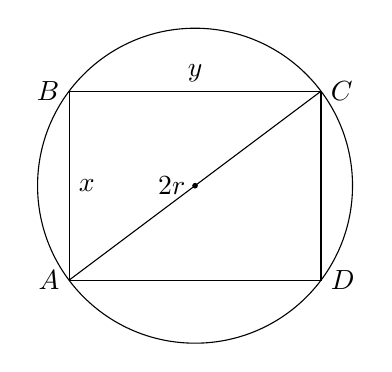
\begin{tikzpicture}[scale=.8]
\draw(0,0)node[left]{$A$}--node[right]{$x$}(0,3)node[left]{$B$}--node[above]{$y$}(4,3)node[right]{$C$}--(4,0)node[right]{$D$}--cycle;
\draw(2,1.5)circle(2.5);
\draw(0,0)--node[left]{$2r$}(4,3);
\draw[fill](2,1.5) circle(1pt);

\end{tikzpicture}
\captionof{figure}{}
\end{minipage}


\begin{example}
    内接于圆的矩形中,怎样的矩形面积最大(图
4.26) ?
\end{example}

\begin{solution}
\textbf{解1:} 设矩形$ABCD$的边长$AB=x$, $BC=y$.

则矩形的面积$S=xy$\hfill (1)

又由勾股定理得 $y=\sqrt{4r^2-x^2}$\hfill (2)

我们的目标是求使面积$S$为最大的条件,通常把函数$S$称为“目标函数”。由(1)知,这里的目标函数是二元的(这与例9是不同的)。(2)式给出了这两个“元”之间的关系,通常把(2) 这样的关系式称为“约束条件”。处理这类问题的方法之一是先把约束条件代入目标函数,使其化为一元函数再去求解。

把(2)代入(1)得
\[S=x\cdot \sqrt{4r^2-x^2}\]

因为$S$与$S^2$同时有最大值(为什么要转而考虑$S^2$ 呢?),
而
$S^{2}= x^{2}( 4 r^{2}-x^{2}$, 记$x^2= t$,
则
$$S^{2}= t(4r^{2}- t)$$
因$t$与$(4r^2-t)$的和是定值 $4r^2$, $t>0$, $4r^2-t>0$。由推论2,
当$t=4r^2-t$时,$S^2$有最大值(也就是$S$有最大值), 得$t=
2r^{2}$, 即$x=\sqrt{2}r$。从而$y=\sqrt{2}r$, 即正方形面积为最大.

\textbf{解2:}若设$\angle ACB=\theta$, 则$AB= 2r\sin\theta$, $BC= 2r\cos\theta$, 矩
形面积$S=AB\cdot BC=2r\sin\theta\cdot 2r\cos\theta=2r^{2}\sin2\theta$, 当$2\theta=90^{\circ}$, 
即$\theta=45^{\circ}$时,$S$有最大值。此时$ABCD$是正方形.
\end{solution}

\begin{example}
$\triangle ABC$中$BC$边上有一点$P$, 由$P$引$AB$、$AC$的垂
线,垂足分别是$M$、$N$. 求使
$\triangle MNP$面积为最大时$P$点的位置(图4.27).
\end{example}

\begin{analyze}
    容易看出$A$、$M$、$P$、$N$四点共圆。

    $\therefore\quad \angle MPN+\angle A=180^{\circ}$

记$MP=m$,$NP=n$
\[S_{\triangle MNP}=\frac{1}{2}mn\sin\angle MPN=\frac{1}{2}mn\sin A\]

$\because\quad \angle A$是定角,欲使$S_{\triangle MNP}$
为最大,须使$mn$为最大,而
$m$、$n$是点$P$到$AB$、$AC$两边的距离。

这个问题是求正数$m$、$n$的乘积为最大的条件,因此有可
能利用“平均不等式”去做。为此我们来看
$m+n$是否为常量
呢?通过选几个特殊点试探一下,可知
$m+n\ne $定值。

\begin{minipage}{.45\textwidth}
\centering
\begin{tikzpicture}[scale=1.5]
\tkzDefPoints{0/0/B, 3/0/C, 2/2/A, 1.3/0/P}
\tkzDefPointBy[projection=onto A--B](P) 
\tkzGetPoint{M}
\tkzDefPointBy[projection=onto A--C](P) 
\tkzGetPoint{N}
\draw(A)--(B)--(C)--cycle;
\draw[pattern=north east lines](M)--(N)--node[right]{$n$}(P)--node[left]{$m$}cycle;
\tkzLabelPoints[below](B,P,C)
\tkzLabelPoints[left](M)
\tkzLabelPoints[right](N)
\tkzLabelPoints[above](A)
\tkzMarkRightAngles[size=.1](B,M,P C,N,P)

\end{tikzpicture}
\captionof{figure}{ }
\end{minipage}
\hfill
\begin{minipage}{.45\textwidth}
\centering
\begin{tikzpicture}[scale=1.5]
    \tkzDefPoints{0/0/B, 3/0/C, 2/2/A, 1.3/0/P}
    \draw(A)--(B)--(C)--cycle;
\draw(A)--(P);
\tkzDefPointBy[projection=onto C--B](A) 
\tkzGetPoint{D}
\tkzMarkRightAngles[size=.1](A,D,C)
\tkzLabelPoints[below](B,P,C,D)
\tkzLabelPoints[above](A)
\draw(A)--node[right]{$h$}(D);


\end{tikzpicture}
\captionof{figure}{ }
\end{minipage}

我们转而考虑“广义的和”
$xm+yn$是否是定值($x,y$是两个常数):

因$PM\bot AB$, $PN\bot AC$, 记$|AB|=c$, $|AC|=b$,$\triangle ABC$
的面积为$S$,则$\frac{1}{2}bn+\frac{1}{2}cm=S$
即
\[bn+cm=2S\]
是一个常量,显然$bn\geqslant0$, $cm\geq0$, 
由平均不等式,得
$$\frac{bn+cm}{2}\geq\sqrt{bn\cdot cm}=\sqrt{bc\cdot mn}$$
欲使$mn$为最 大,当且仅 当$nb=mc$时,即$S_{\triangle ACP}=S_{\triangle ABP}$(图4.28)。这两个三角形可看做是同高(都为$h$)、异底($BP$ 与$PC$)的三角形,所以当且仅当$BP=PC$时它们的面积相等。即点$P$位于$BC$的中点时,$\triangle MNP$的面积为最大。
\end{analyze}

\begin{thm}
  {思考题} 对此例,你还能想到别的解法吗(如以参数体
现$P$为动点)?  
\end{thm}

\begin{example}
    常见的食品罐头盒的形状大多是正圆柱体(图4.29), 要制造容积一定的罐头盒,它的高和底面半径多大时,用料最省(表面积最小)?
\end{example}

\begin{figure}[htp]
    \centering
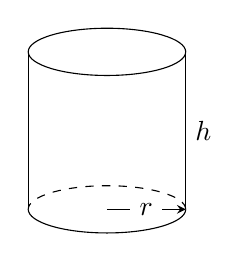
\begin{tikzpicture}[>=stealth]
% \draw(0,0) ellipse(1 and .3);
\draw(0,2) ellipse(1 and .3);
\draw(-1,0)--(-1,2);
\draw(1,0)--node[right]{$h$}(1,2);
\draw[->](0,0)--node[fill=white]{$r$}(1,0);
\draw[dashed](1,0) arc (0:180:1 and .3);
\draw(1,0) arc (0:-180:1 and .3);

\end{tikzpicture}
    \caption{}
\end{figure}

\begin{solution}
设罐头盒的高为$h$, 底面圆的半径为$r$, 则
容积
$V=\pi r^2 h$\hfill (1)

表面积$S=2\pi r^2+2\pi rh$\hfill (2)

现在的问题是:$V$为定值,$h$、$r$多大时(或$h$与$r$的比为
多大时)能使$S$取得最小值。

我们把约束条件(1)代入目标函数(2), 得
\[S=2\pi r^2+\frac{2V}{r}\]
将此式变形为
\[S=2\pi r^2+\frac{V}{r}+\frac{V}{r}\ge 3\sqrt[3]{2\pi r^2\cdot \frac{V}{r}\cdot \frac{V}{r}}=3\sqrt[3]{2\pi V^2}\]
上式取最小值的条件是$2\pi r^2=\frac{V}{r}$
,即
\[r=\sqrt[3]{\frac{V}{2\pi}}=\frac{1}{2\pi}\sqrt[3]{4\pi^2 V}\]
代入(1)得
\[h=\frac{1}{\pi}\sqrt[3]{4\pi^2 V}\]
由此可得$h=2r$.

所以,当盒子的高与底面圆的直径相等时用料最省。
\end{solution}



\section*{习题十六}
\begin{center}
    \bfseries A
\end{center}

\begin{enumerate}
    \item 求下列函数的最小值:
\begin{enumerate}[(1)]
    \item $y=\frac{2x^2-2x+1}{2x},\quad (x>0)$
    \item $y=\frac{2(x-1)^2+5}{x-1},\quad (x>1)$
\end{enumerate}

\item 证明:周长等于定值的矩形中,面积以正方形的为最大.

\item 求下列函数的最大值:
\begin{enumerate}[(1)]
    \item $y=2x\sqrt{100-x^2}\quad (x>0)$
    \item $y=x(3-2x)^2$
    \item $M=3\sin\alpha \cdot \cos^2\alpha \quad \left(0<\alpha<\frac{\pi}{2}\right)$
\end{enumerate}

\item 把40分成两个数,欲使这两个数的平方和为最小,应如
何分?
\item 要用篱笆围一个面积为1600平方米的矩形养鸡场,求篱
笆至少需要多长?
\end{enumerate}

\begin{center}
    \bfseries B
\end{center}

\begin{enumerate}\setcounter{enumi}{5}
    \item 有一批木板可围成长200米的围墙。现在打算用来围一个
    矩形场地,而一边利用工厂的墙作为天然屏障。问采用怎
    样的围法可使场地的面积最大?
    \item 已知等腰梯形周长为60cm, 底角为$60^{\circ}$. 问这个梯形边
    长为多少时面积最大?
    \item 直角三角形的斜边为定长$c$, 求这个直角三角形面积的最
    大值,并指出取得最大值的条件。
    \item 某溢洪闸门水道截面形状
    如图4.30所示,面积为$S$, 在
    什么条件下这个截面的周
    长最短?
    \item 在半径为$R$的球的所有外
    切圆锥中,求全面积最小的一个。
    \item 某工厂要制造一个无盖的圆柱形桶。它的容积是$\frac{3}{2}\pi$立方米。用来做底的金属每平方米价格3元,做侧面的
    金属每平方米价格2元。按照怎样的尺寸来制造这个圆
    桶,才能使得成本最低?
\end{enumerate}

\begin{figure}[htp]
    \centering
\begin{tikzpicture}[>=stealth, scale=.7]
\draw(-2,0)--(2,0)--(2,3) arc (0:180:2)--(-2,0);
\draw[dashed](-3,3)--(3,3);
\draw[dashed](0,-1)--(0,6);
\draw[<->](2.5,0)--node[fill=white]{$h$}(2.5,3);
\draw(2,0)--(3,0);
\draw[->](0,3)--node[left]{$r$}+(60:2);
\end{tikzpicture}
    \caption{}
\end{figure}

\section{本章小结}
\subsection*{知识结构分析}
本章共有五个部分:
\begin{enumerate}
    \item \textbf{不等式的概念与性质}:  这是本章的基础,也是学好
本章的关键。对此4.3节已做了小结。
\item \textbf{不等式的证明方法}: 这是本章的重点。讲了四种证
法和四个专题。四种证法是:
\begin{enumerate}[(1)]
\item 比较法(作差法和作商法)——这是证明不等式
的最基本、最常用的方法;
\item 分析法和综合法(这是论证的一般方法,在这里被用来证明不等式);
\item 放缩法——这是证明不等式或估值的特定方法。
\end{enumerate}

对于这四种方法,要弄清每一种方法适用的对象(证明
哪一类不等式)、原理、主要步骤(包括技巧)和表达方法
(格式)。

四个专题是:
\begin{enumerate}[(1)]
\item 用平均不等式证不等式;
\item 附有条件的不等式的证法;
\item 平方平均数;
\item 柯西不等式。
\end{enumerate}

对这四个专题,要掌握每一专题适用的对象和主要技
巧。如用“平均”法证不等式,对象是形如“和的形式≥积的
形式”这一类不等式,以及几个这种不等式的“迭加”或“迭
乘”。主要技巧包括:(a)“和的形式”与“积的形式”的识
别;(b)字母轮换式的识别等。

\item \textbf{不等式的解法}: 这也是本章的重点内容。
\begin{enumerate}[(1)]
\item 一元一次、二次不等式的解法;
\item 一元高次不等式的解法;
\item 分式不等式的解法——化归解整式不等式;
\item 无理不等式的解法——化归解有理不等式;
\item 指数对数不等式的解法——化归解代数不等式。
\end{enumerate}

\item \textbf{绝对值不等式的性质、证明和解法}: 这部分讲的都
是基本知识,对以后的学习用途甚大,应当很好地掌握。
\item \textbf{利用平均不等式求函数的最大值或最小值}: 这也是
本章的重点。其中,正确地理解推论中的条件至关重要。它
是掌握和运用有关变形技巧的基础。

\end{enumerate}


\subsection*{本章应着重掌握的数学思想和方法}
\begin{enumerate}
\item \textbf{通过对不等式性质及证明方法的学习,掌握比较法、
分析法、综合法、放缩法等几种推理论证的方法}:  要能根据
题目的特点,恰当地选取证明的方法,提高思维能力和逻辑
推理能力。
\item \textbf{数形结合的方法}: 借助函数图象讨论不等式解的各种
情况及借助数轴确定不等式(组)的解是解不等式的重要方
法。
\item \textbf{化归的思想}: 为了用好化归的思想,关键是掌握好转化的条件,以达到化归的目的。
\end{enumerate}

\section*{复习题四}
\begin{center}
    \bfseries A
\end{center}

\begin{enumerate}
\item 若$a,b\in \R^+$, 比较$a^3-b^3$与$3a^2(a-b)$的大小。
\item 若$a,b\in \R^+$, 试比较$\left(\frac ba\right)^n$与$\left(\frac ab\right)^{n+1}$的大小,$(n\in \N).$

\item 若$a>b>c>0$, 依照从小到大的次序用“$<$”号连接下列
各式:
$$a,\quad c,\quad \frac{a+b+c}3,\quad \sqrt[3]{abc},\quad \sqrt[3]{\frac{a^2+b^2+c^2}3}$$
\item 若$a,b\in \R^+$, 求证
$$\frac{1}{a^5}+\frac{1}{b^5}\leqslant\frac{\sqrt{b}}{a^5\sqrt{a}}+\frac{\sqrt{a}}{b^5\sqrt{b}}.$$
\item 对于$n\in\mathbb{N}$, 试证
$$2\sqrt{n+1}-2\sqrt{n}<\frac{1}{\sqrt{n}}<2\sqrt{n}-2\sqrt{n-1}.$$
\item 若$a,b,c\in \R^+$, 求证
$$(a+b+c)^{3}(a^{2}+b^{2}+c^{2})^{3}(a^{3}+b^{3}+c^{3})\geq 2187a^{4}b^{4}c^{4}$$

\item 若$x\in \R^+$, 且$x\neq1$, $n\in\mathbb{N}$, 求证
$$(1+x^n)(1+x)^n>2^{n+1}x^n$$
\end{enumerate}

\begin{center}
    \bfseries B
\end{center}

\begin{enumerate}\setcounter{enumi}{7}
    \item 若$a,b,c,d\in \R$, 且$a^{2}+b^{2}=1$, $c^{2}+d^{2}=1$,
    
求证:$-\frac14\leq abcd\leqslant\frac14$.

\item 已知$n\in\mathbb{N}$, 求证
$$\sqrt{2}+\sqrt{6}+\sqrt{12}+\cdots+\sqrt{n(n+1)}<\frac{n(n+2)}{2}.$$
\item 若$a,b\in \R^+$, 且$ab-(a+b)=1$,
求$a+b$的最小值。

\item 若$a,b,c$是三角形的三个边,求证
$$\frac1{a+b-c}+\frac1{b+c-a}+\frac1{c+a-b}>\frac9{a+b+c}.$$
\item 若$a$、$b,c\in \R^+$,且两两不等,求证
$$2(a^3+b^3+c^3)>a^2(b+c)+b^2(c+a)+c^2(a+b) $$
\item 若$a,b,c\in\mathbb{N}$, 求证$ab+bc+ca\leqslant3abc.$

\item 若$a,b,c\in \R^+$, 求证
$$a^ab^bc^c\geqslant(abc)^{\tfrac{a+b+c}3}\geqslant a^{\tfrac{b+c}2}b^{\tfrac{c+a}2}c^{\tfrac{a+b}2}.$$
\item 若$a,b,c\in \R^+$, 求证
$$\log_3(a^2+b^2+c^2)-2\log_3(a+b+c)\geqslant-1 $$
\item 已知$\frac{a_{1}}{b_{1}}<\frac{a_{2}}{b_{2}}<\cdots<\frac{a_{m}}{b_{m}}$ 且所有的字母都表示正数。求
证
$$\frac{a_1}{b_1}<\frac{a_1+a_2+\cdots+a_n}{b_1+b_2+\cdots+b_n}<\frac{a_n}{b_n}$$
\item 已知$\sqrt[m]{a}<\sqrt[n]{b}<\sqrt[p]{c}<\sqrt[q]{d}$, 其中$a,b,c,d$都可
是正数,$m,n, p,q$ 都是正整数,求证
$$\sqrt[m]{a}<\sqrt[{m+n+p+q}]{abcd}<\sqrt[q]{d}$$
\item 若$p^3+q^3=2$, $p,q$为正数,求证$p+q\leqslant2$.
\item \begin{enumerate}[(1)]
\item 证明$m=\frac12 \cdot \frac34\cdot \frac56\cdots\frac{2n-1}{2n}\cdots \frac{99}{100}<\frac1{10};$
\item 对此题你还能加以推广吗?
\end{enumerate}

\item 在直角三角形$AB$C中,$a$、$b$是直角边,$c$是斜边,$r$是内切圆半径,$h$为斜边上的高,求证
\begin{multicols}{2}
\begin{enumerate}[(1)]
    \item $c\geqslant \frac {a+ b}{\sqrt {2}}$;
    \item  $r\leqslant \frac c2 ( \sqrt {2}- 1 )$ .
\end{enumerate}    
\end{multicols}

\end{enumerate}

\begin{center}
    \bfseries C
\end{center}

\begin{enumerate}\setcounter{enumi}{20}
    \item 在$\triangle ABC$中,$A+C=2B$成等差数列,且$b=1$,
    
求证:$1<a+c\leqslant2$

\item 若$a_{1}^{2}+ a_{2}^{2}+ \cdots + a_{n}^{2}= 1$ , $x_{1}^{2}+ x_{2}^{2}+ \cdots + x_{n}^{2}= 1$

求证: $-1\leqslant a_1x_1+a_2x_2+\cdots+a_nx_n\leqslant1$
\item 设$f(x)=\lg\frac{1+2^{x}+4^{x}a}{3}$, 其中$a\in \R$,
\begin{enumerate}[(1)]
    \item 若$0<a\leqslant1$, 求证:当$x\neq0$时,有
    $2f(x)=f(2x)$
    \item 如果当$x\in(-\infty,1)$时$f(x)$有意义,求$a$的取值
    范围。
\end{enumerate}

\end{enumerate}